% =============================================================
% Section 4: Results
% =============================================================
\section{Results}\label{sec:results}

The three models are presented in a uniform format: field
accuracy against the FD reference (snapshots, pointwise error,
and summary metrics), the ringdown waveform at the observer,
and the QNM extraction table of the five methods of
Sec.~\ref{sec:qnm-methods} under the reporting convention of
Sec.~\ref{sec:reporting}. Sections~\ref{sec:res-repro}%
--\ref{sec:res-fwd} treat one black hole at a time
(reproduction, enhanced forward);
Sec.~\ref{sec:res-hyb} evaluates the hybrid
surrogate on the canonical BH and on a $100$-BH test
population; and Sec.~\ref{sec:res-kerr} generalises the hybrid
to a population of rotating (Kerr) black holes. Supporting
scans and diagnostics are
collected in Appendix~\ref{app:supp}.
Table~\ref{tab:results-summary} summarises the principal
quantitative results of the three Schwarzschild models; the
Kerr generalisation is summarised separately in
Table~\ref{tab:kerr-summary}.

\begin{table}[!htbp]
\centering
\caption{Summary of the principal quantitative results.
Field errors are computed against the FD reference over the
full $(x,t)$ grid: RMSD in field units
($|\Phi|_{\max} \approx 1$) and relative $L^{2}$ norm (RL2).
QNM errors are relative errors against the Leaver
continued-fraction values $M\omega_{0} = 0.3737$,
$\tau_{0}/M = 11.241$, under the reporting convention of
Sec.~\ref{sec:reporting}: each entry is the smallest error over
the M1--M5 estimator suite of Sec.~\ref{sec:qnm-methods} --- the
Leaver-closest of five extractors, none of which sees the
reference during extraction --- labelled with the estimator
used; the per-estimator breakdown is in
Tables~\ref{tab:repro-qnm}, \ref{tab:fwd-qnm}
and~\ref{tab:hyb-canonical}. All QNM errors are read at the common
observer $\xq = 10\,M$ (window $[10,50]\,M$ for the PINN rows,
$[10,100]\,M$ for the hybrid).
Population-row QNM
errors are medians over the $100$-BH test set; the hybrid
population field entries are population means. For the reproduction rows
the corresponding values in \citet[Table~2]{Patel2024pinn} are
$\mathrm{RL2} = 28.06\%$ (Zerilli) and $23.59\%$
(Regge--Wheeler); for the hybrid rows the coarse-up baseline
gives $\mathrm{RL2} = 4.93\%$ (canonical) and $6.11\%$
(population). Dashes denote quantities not applicable to,
or not evaluated for, that row.}
\label{tab:results-summary}
\footnotesize
\setlength{\tabcolsep}{4pt}
\renewcommand{\arraystretch}{1.15}
\begin{tabular}{@{}lllcccc@{}}
\toprule
Sec. & Model & Evaluation & Field RMSD & RL2 [\%]
     & $|\Delta\omega|/\omega$ [\%] & $|\Delta\tau|/\tau$ [\%] \\
\midrule
\ref{sec:res-repro} & Reproduction (Zerilli)       & canonical BH             & $1.83\times 10^{-3}$ & $1.30$  & $1.08$~(M1)  & $1.50$~(M2)  \\
\ref{sec:res-repro} & Reproduction (Regge--Wheeler) & canonical BH            & $3.77\times 10^{-3}$ & $2.67$  & $0.56$~(M1)  & $1.56$~(M2)  \\
\ref{sec:res-fwd}   & Enhanced forward PINN        & canonical BH             & $8.17\times 10^{-4}$ & $0.58$  & $0.029$~(M4) & $1.99$~(M2)  \\
\ref{sec:res-hyb}   & Hybrid surrogate             & canonical BH             & $6.28\times 10^{-4}$ & $0.445$ & $0.047$~(M5) & $1.34$~(M1)  \\
\ref{sec:res-hyb}   & Hybrid surrogate             & $100$-BH population      & $9.68\times 10^{-4}$ & $0.648$ & $0.152$~(M4) & $0.528$~(M4) \\
\bottomrule
\end{tabular}
\end{table}

% --------------------------------------------------------------
\subsection{Faithful reproduction of the prior-work baseline}
\label{sec:res-repro}

We first establish that the pipeline reproduces the prior-work
baseline of \citet{Patel2024pinn} --- the only previous
time-domain PINN treatment of these $\ell = 2$ master
equations --- before any methodological change is introduced;
it does, improving on the published field errors by an order
of magnitude. The forward PINN is trained at their exact
settings (Table~\ref{tab:fwd-hyper}: uniform collocation
resampling, their loss weights and optimiser budget), i.e.\
without the enhancements of Sec.~\ref{sec:res-fwd}, on both
the even-parity (Zerilli) and odd-parity (Regge--Wheeler)
potentials.

\paragraph{Field accuracy.} At matched settings the
reproduction reaches $\mathrm{RL2} = 1.30\%$
(RMSD $1.83\times 10^{-3}$) on the Zerilli potential and
$\mathrm{RL2} = 2.67\%$ (RMSD $3.77\times 10^{-3}$, MAD
$2.53\times 10^{-3}$) on the Regge--Wheeler potential, against
$28.06\%$ and $23.59\%$ respectively in
\citet[Table~2]{Patel2024pinn} --- a factor of $\sim\!21$
(Zerilli) and $\sim\!9$ (Regge--Wheeler) at identical
architecture, loss weights and optimiser budget; the remaining
differences are implementation-level (double-precision
training and the outgoing-pulse initial velocity of
Sec.~\ref{sec:fwd-pinn}).
Snapshot overlays and global error maps are shown in
Figs.~\ref{fig:repro-zer-field} and~\ref{fig:repro-rw-field},
and the training histories in Fig.~\ref{fig:repro-loss}.

\begin{figure}[!htbp]
\centering
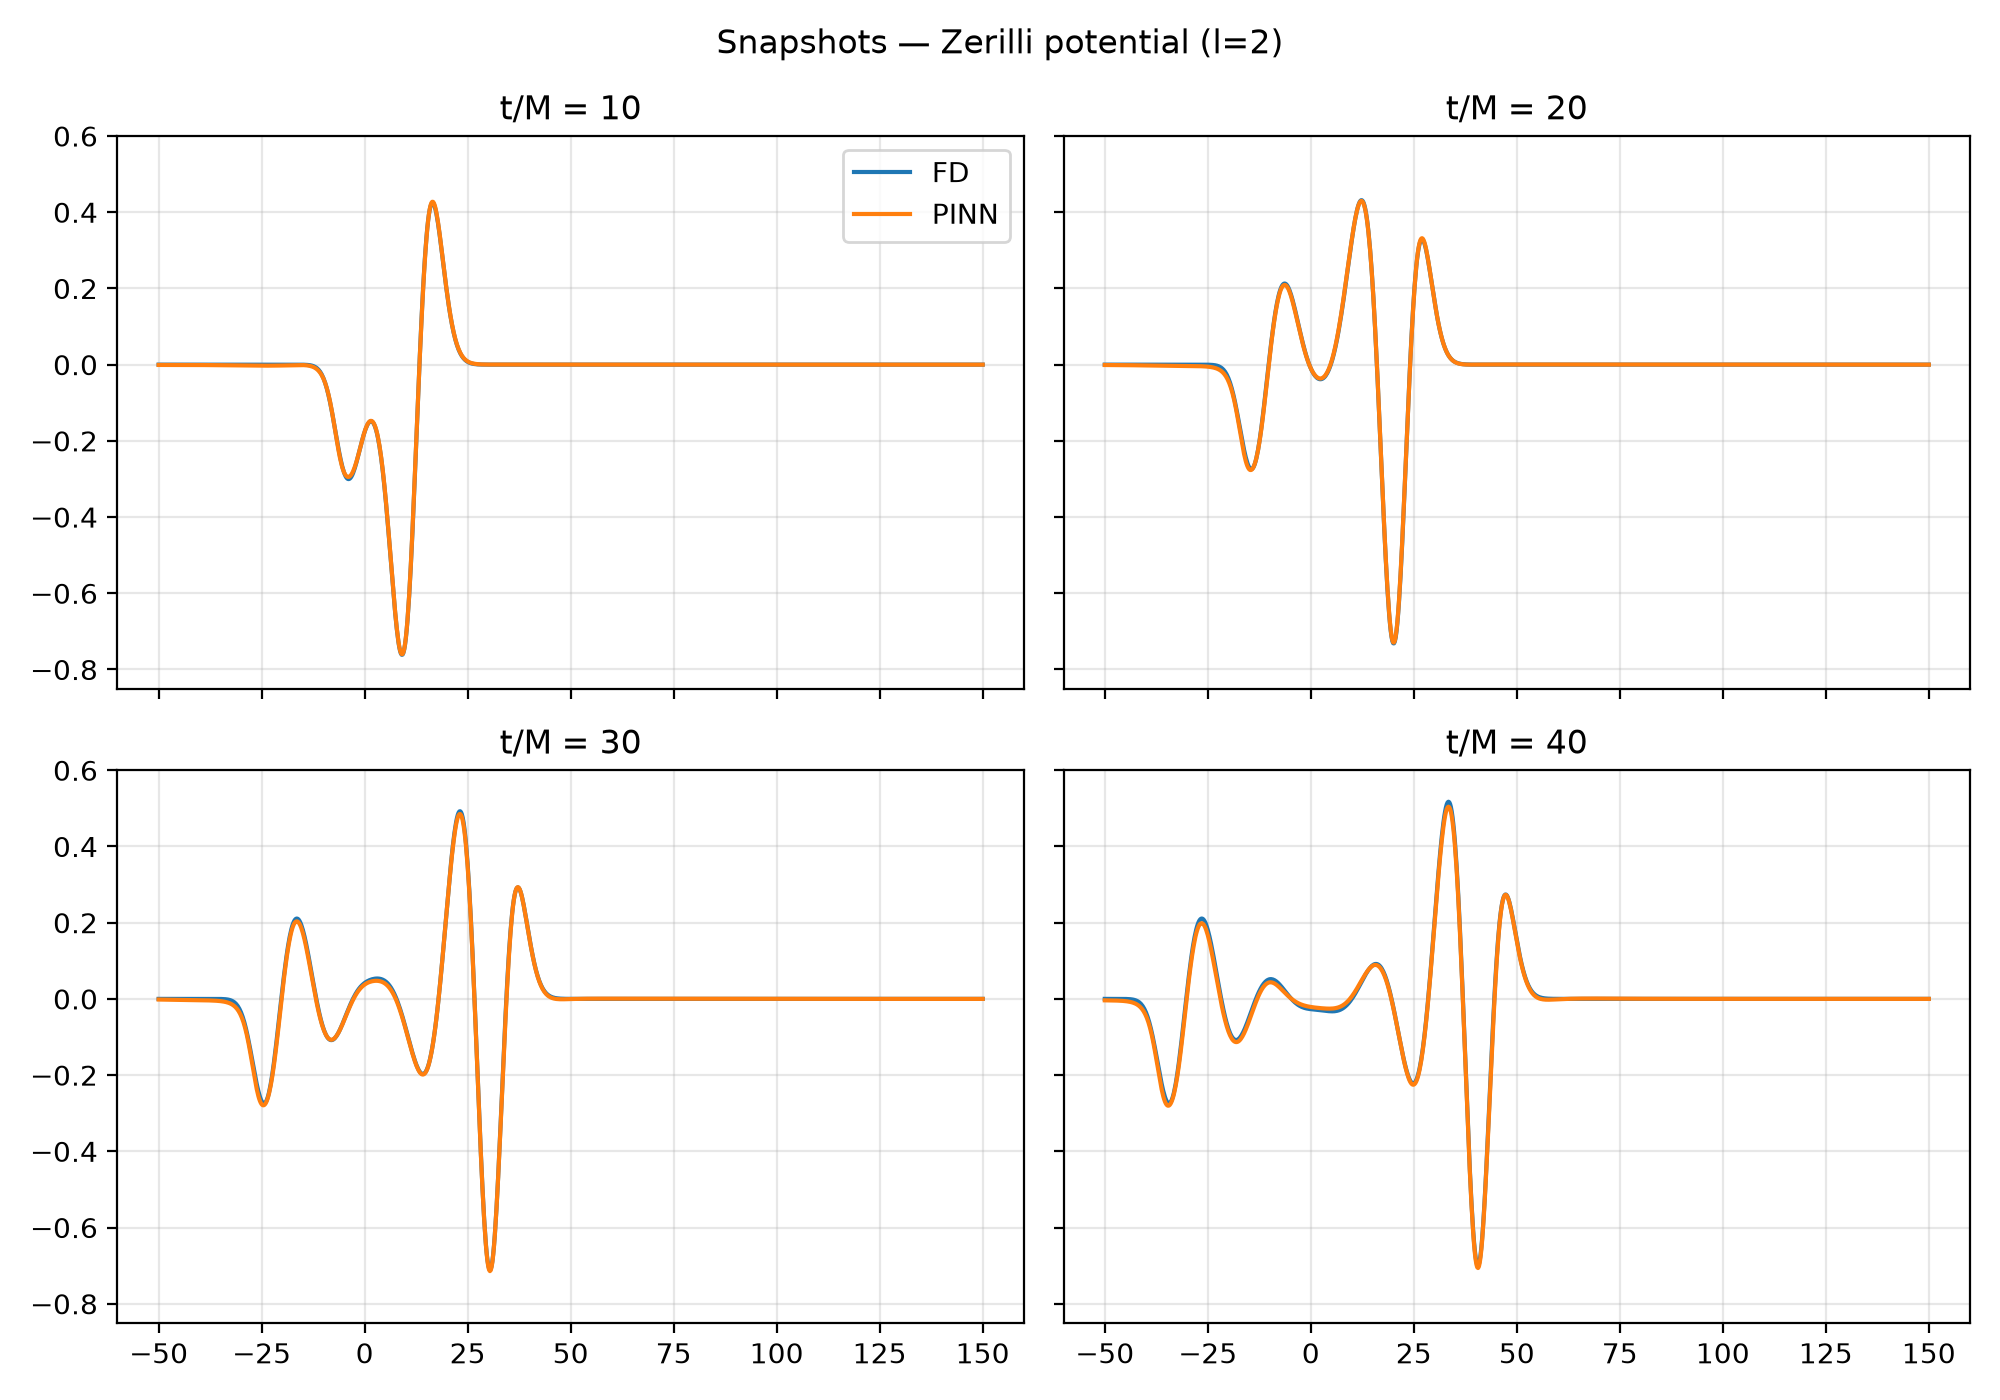
\includegraphics[width=0.82\textwidth]{../outputs/pinn/zerilli_l2_paper/snapshots.png}\\[0.4em]
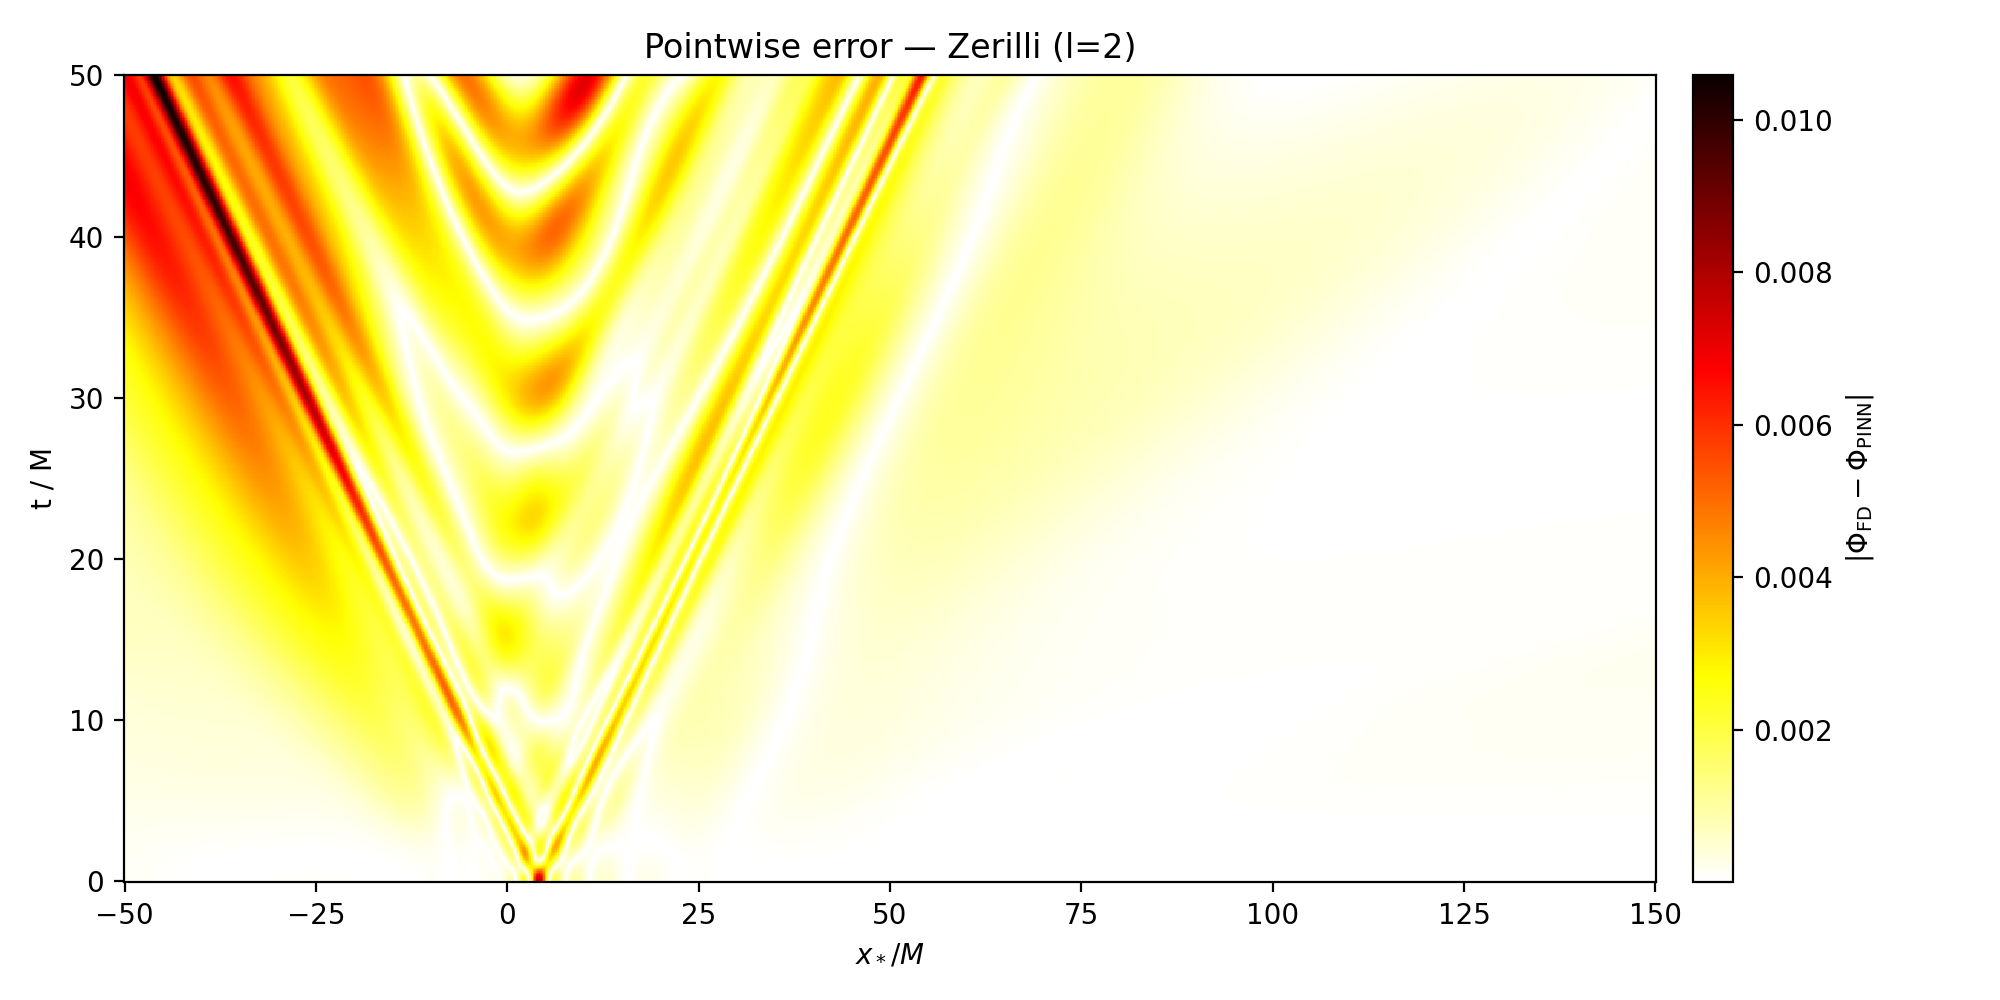
\includegraphics[width=0.88\textwidth]{../outputs/pinn/zerilli_l2_paper/error_heatmap.png}
\caption{Faithful reproduction on the Zerilli potential. Top:
snapshots of $\Phi(x,t)$ at $t/M \in \{10,20,30,40\}$ overlaid
for the reproduced PINN and the FD reference; the curves are
visually indistinguishable on this scale. Bottom: global
pointwise error $|\Phi_{\mathrm{FD}} - \Phi_{\mathrm{PINN}}|$
on $x \in [-50,150]\,M$, $t \in [0,50]\,M$, peaking at
$\sim\!1.0\times 10^{-2}$ on the outgoing wavefront,
consistent with the gridwise RMSD of $1.83\times 10^{-3}$.}
\label{fig:repro-zer-field}
\end{figure}

\begin{figure}[!htbp]
\centering
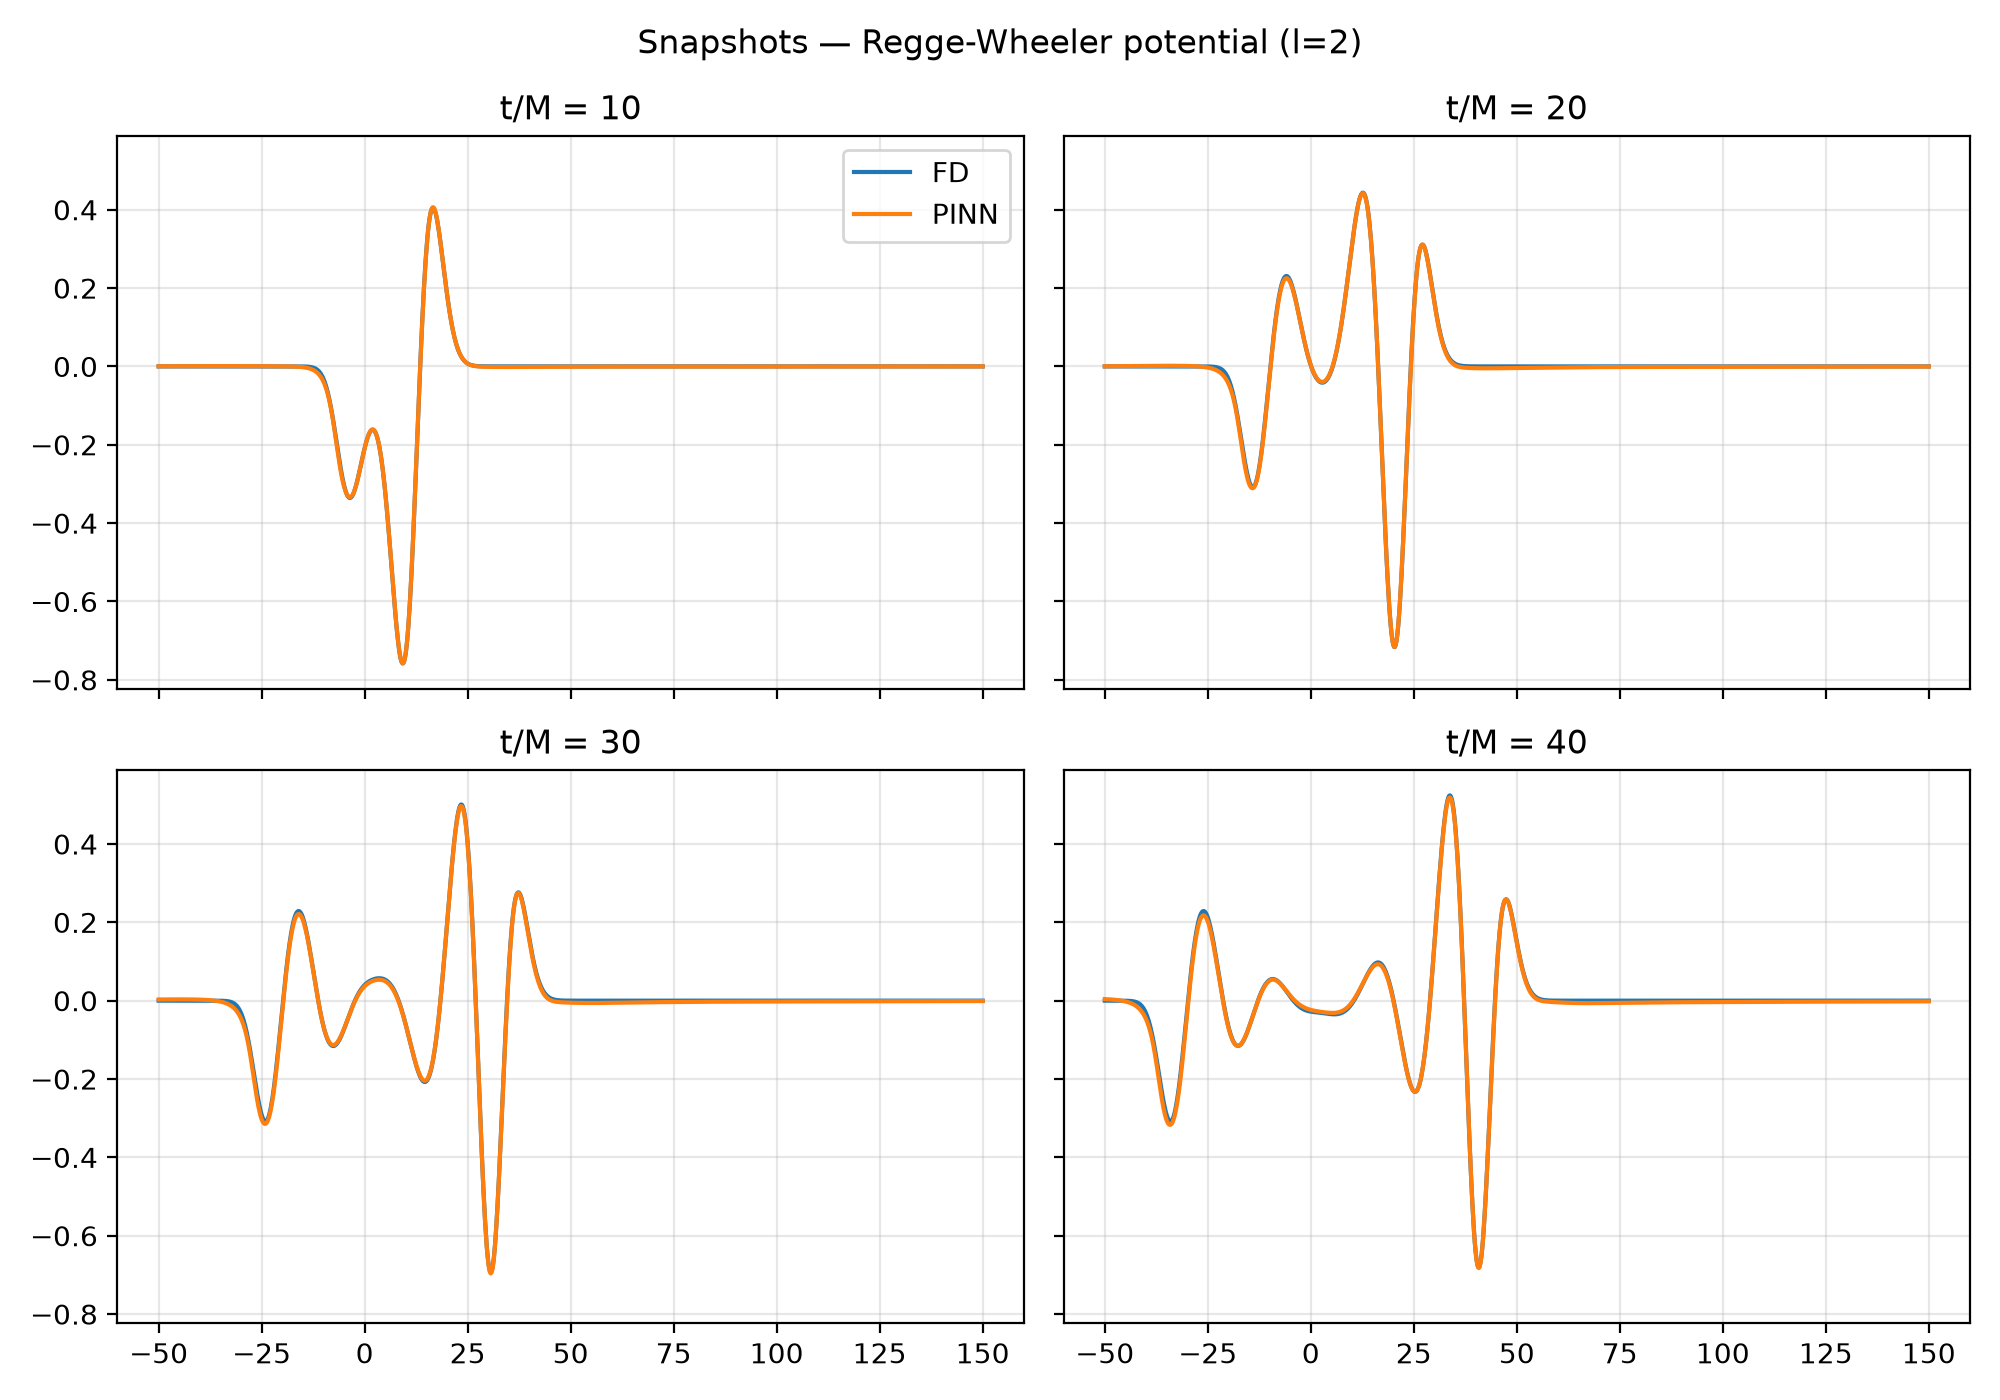
\includegraphics[width=0.82\textwidth]{../outputs/pinn/regge_wheeler_l2_paper/snapshots.png}\\[0.4em]
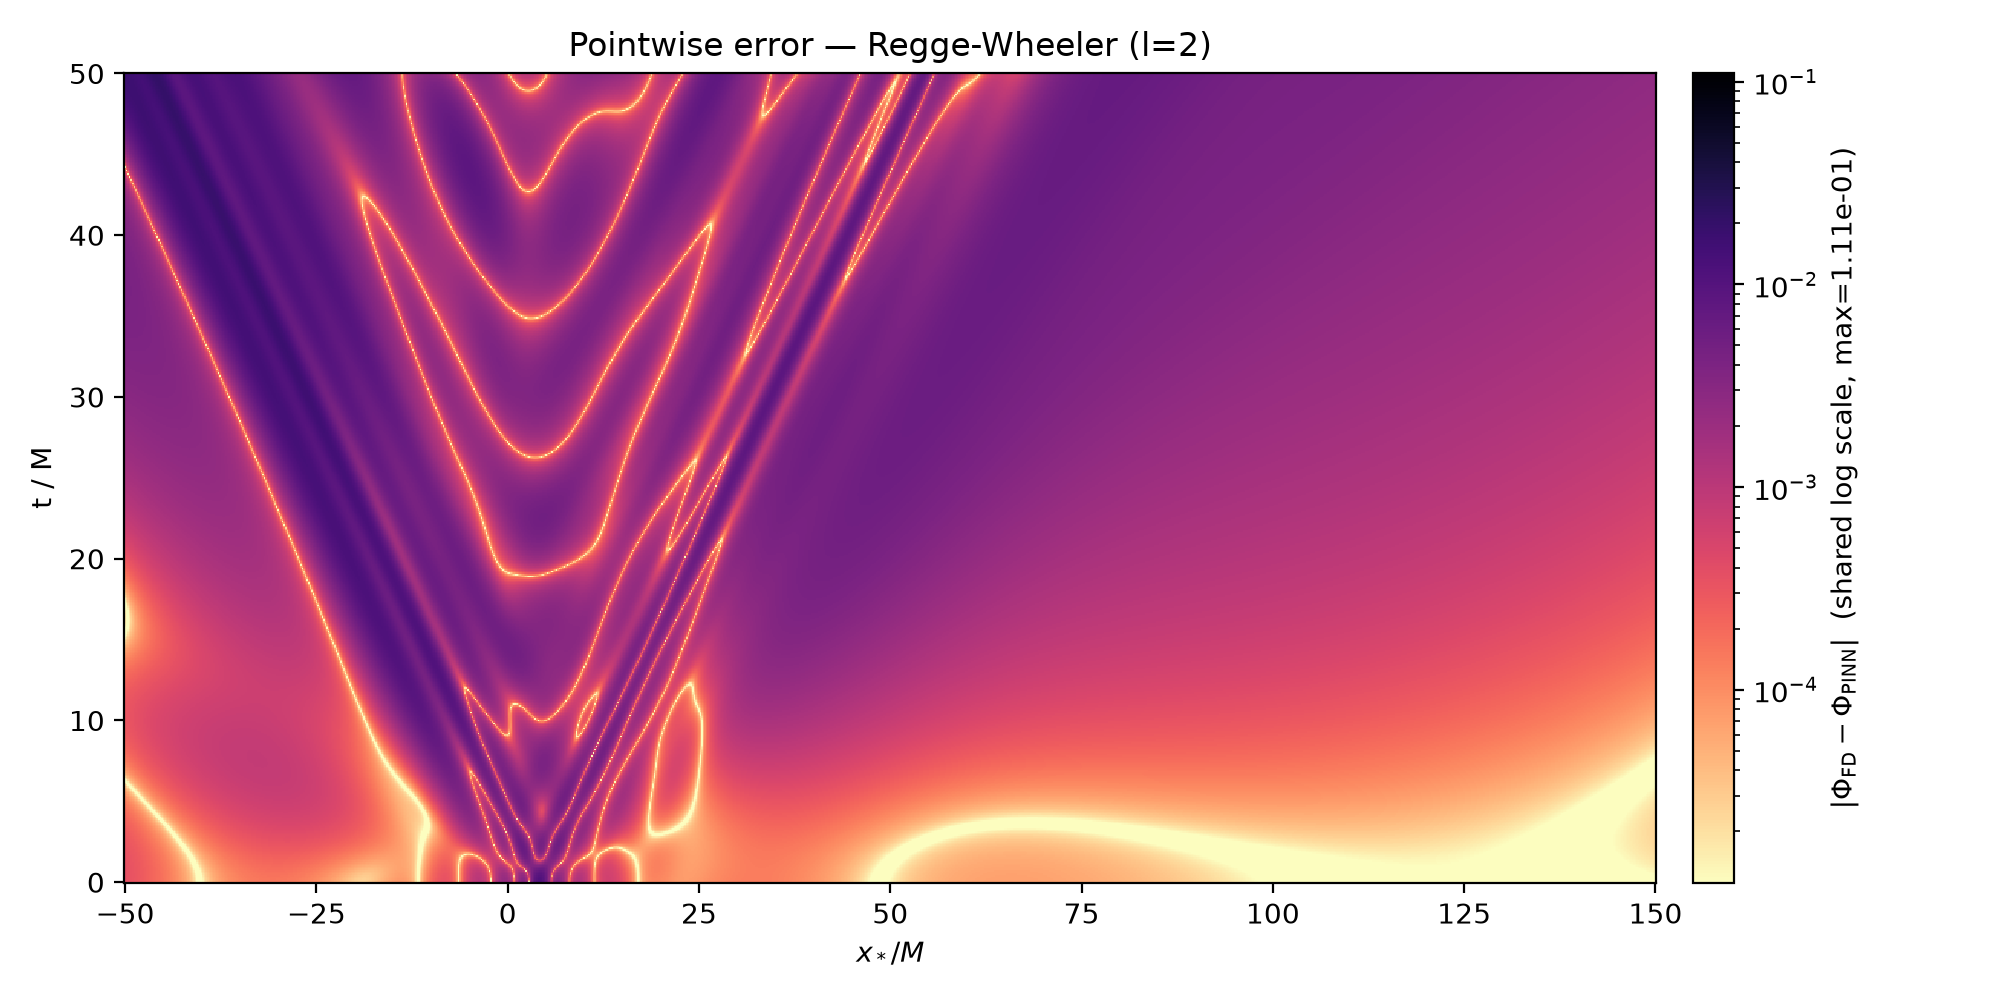
\includegraphics[width=0.88\textwidth]{../outputs/pinn/regge_wheeler_l2_paper/error_heatmap.png}
\caption{Faithful reproduction on the Regge--Wheeler potential.
Top: snapshots of $\Phi(x,t)$ at $t/M \in \{10,20,30,40\}$
overlaid for the reproduced PINN and the FD reference. Bottom:
global pointwise error $|\Phi_{\mathrm{FD}} - \Phi_{\mathrm{PINN}}|$
on the same domain, concentrated on the left-going late-time
characteristic, consistent with the gridwise RMSD of
$3.77\times 10^{-3}$.}
\label{fig:repro-rw-field}
\end{figure}

\paragraph{QNM extraction.} Table~\ref{tab:repro-qnm} applies
the two extraction methods used by \citet{Patel2024pinn} (M1
and M2, their ``PINN1''/``PINN2'') to the reproduced fields at
$\xq = 10\,M$. The frequencies agree at the one-to-two-percent
level on both potentials; the damping time, the observable most
sensitive to field quality, improves several-fold: from
$14.42\%$ to $1.50\%$ (Zerilli) and from $5.39\%$ to $1.56\%$
(Regge--Wheeler, M2). The ringdown at the observer, with the
damped-cosine reconstructions overlaid, is shown in
Figs.~\ref{fig:repro-zer-ringdown}
and~\ref{fig:repro-rw-ringdown}.

\begin{table}[!htbp]
\centering
\caption{Faithful reproduction: QNM extraction at $\xq = 10\,M$
with the two methods of \citet{Patel2024pinn} (M1 = FFT $+$
log-envelope, M2 = damped-cosine NLS; their PINN1/PINN2),
applied to the reproduced PINN fields on both potentials.
Reference values are the Leaver continued-fraction Schwarzschild
$\ell = 2$ fundamental $M\omega_0 = 0.3737$,
$\tau_0/M = 11.241$; \citet{Patel2024pinn} quote their
percentage errors against the rounded reference
$M\omega_0 = 0.374$. Bold entries mark the damping-time
improvement discussed in the text.}
\label{tab:repro-qnm}
\footnotesize
\setlength{\tabcolsep}{4pt}
\renewcommand{\arraystretch}{1.1}
\begin{tabular}{@{}llcccc@{}}
\toprule
 & & \multicolumn{2}{c}{This work} & \multicolumn{2}{c}{\citet{Patel2024pinn}} \\
\cmidrule(lr){3-4}\cmidrule(l){5-6}
Potential & Method & $M\omega$ (err) & $\tau/M$ (err) & $M\omega$ (err) & $\tau/M$ (err) \\
\midrule
Zerilli & M1 & $0.3697$ ($1.08\%$) & $10.671$ ($5.07\%$) & $0.375$ ($0.29\%$) & $10.089$ ($10.25\%$) \\
Zerilli & M2 & $0.3784$ ($1.25\%$) & $11.410$ ($\mathbf{1.50\%}$) & $0.376$ ($0.52\%$) & $9.620$ ($14.42\%$) \\
Regge--Wheeler & M1 & $0.3716$ ($0.56\%$) & $10.753$ ($4.34\%$) & $0.373$ ($0.11\%$) & $10.474$ ($6.82\%$) \\
Regge--Wheeler & M2 & $0.3811$ ($1.97\%$) & $11.416$ ($\mathbf{1.56\%}$) & $0.383$ ($2.51\%$) & $10.636$ ($5.39\%$) \\
\bottomrule
\end{tabular}
\end{table}

\begin{figure}[!htbp]
\centering
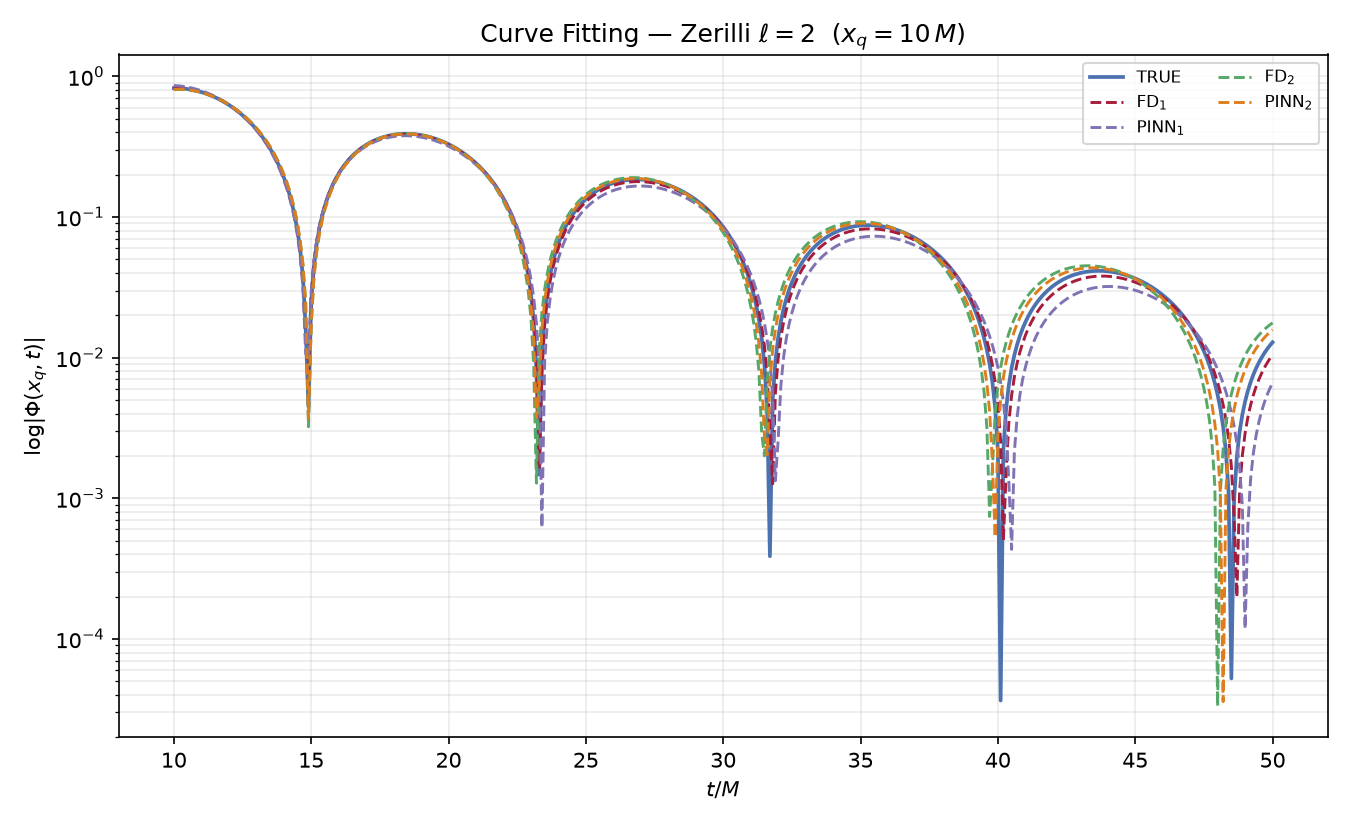
\includegraphics[width=0.80\textwidth]{../outputs/pinn/zerilli_l2_paper/curve_fitting.png}
\caption{Faithful reproduction on the Zerilli potential:
ringdown at the observer. $\log_{10}|\Phi(\xq{=}10\,M, t)|$ for
the reproduced PINN and FD waveforms with the damped-cosine
reconstructions of the M1 and M2 extractions of
Table~\ref{tab:repro-qnm} overlaid.}
\label{fig:repro-zer-ringdown}
\end{figure}

\begin{figure}[!htbp]
\centering
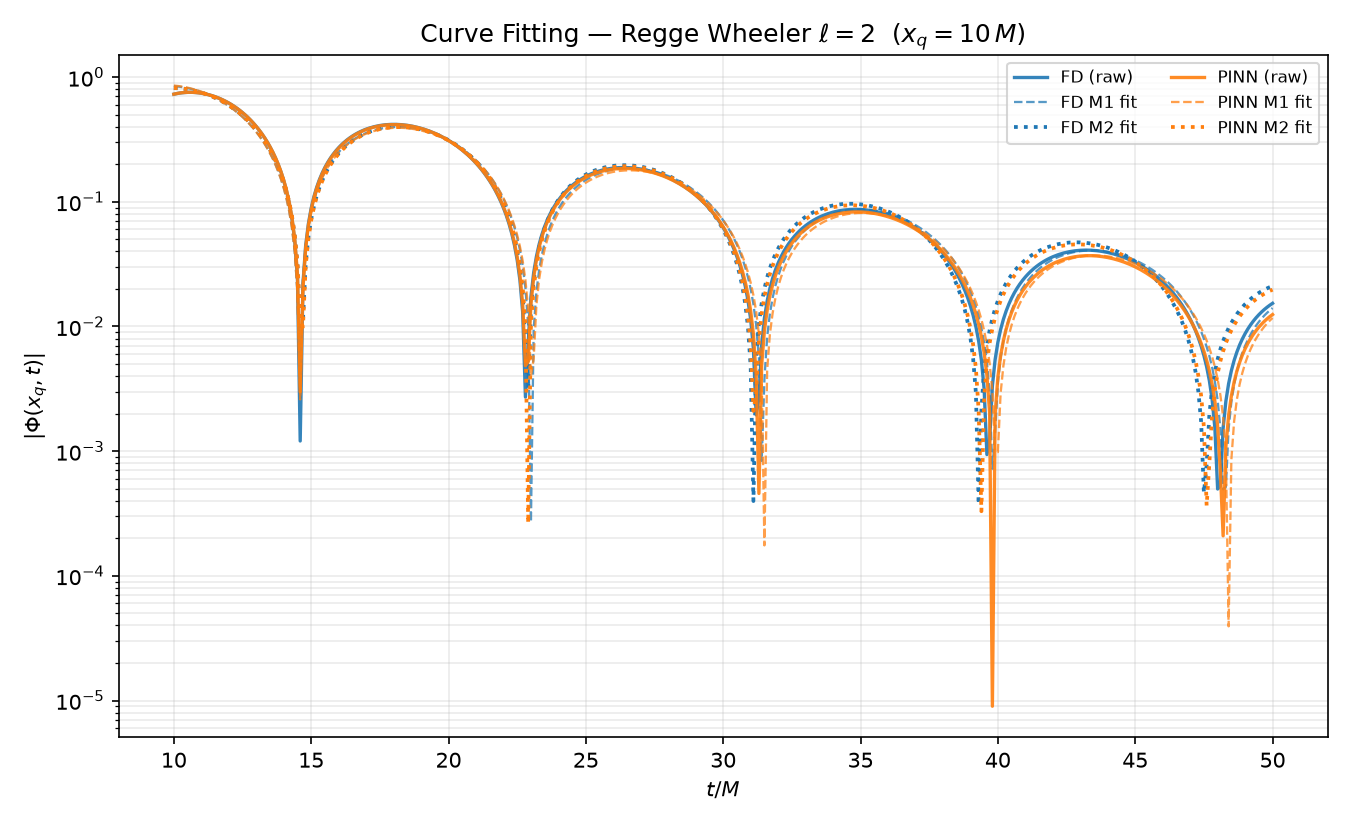
\includegraphics[width=0.80\textwidth]{../outputs/pinn/regge_wheeler_l2_paper/curve_fitting.png}
\caption{Faithful reproduction on the Regge--Wheeler potential:
ringdown at the observer. $\log_{10}|\Phi(\xq{=}10\,M, t)|$ for
the reproduced PINN and FD waveforms with the damped-cosine
reconstructions of the M1 and M2 extractions of
Table~\ref{tab:repro-qnm} overlaid.}
\label{fig:repro-rw-ringdown}
\end{figure}

\begin{figure}[!htbp]
\centering
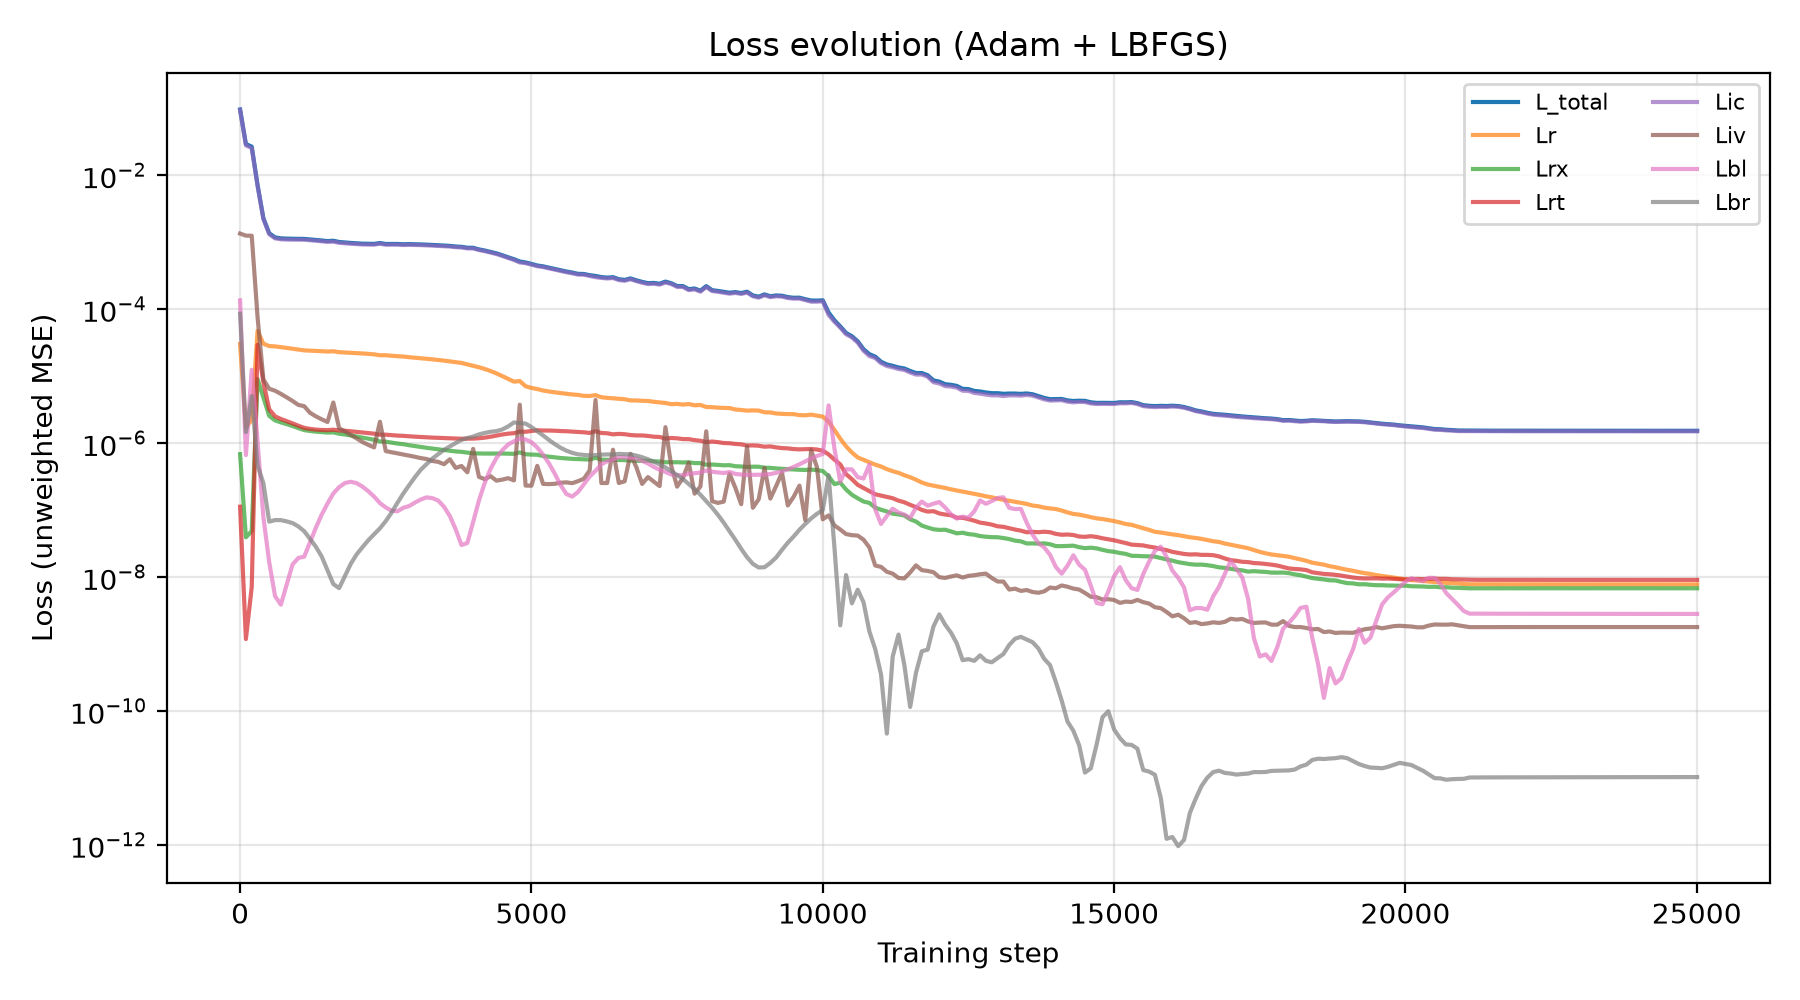
\includegraphics[width=0.80\textwidth]{../outputs/pinn/zerilli_l2_paper/loss.png}\\[0.4em]
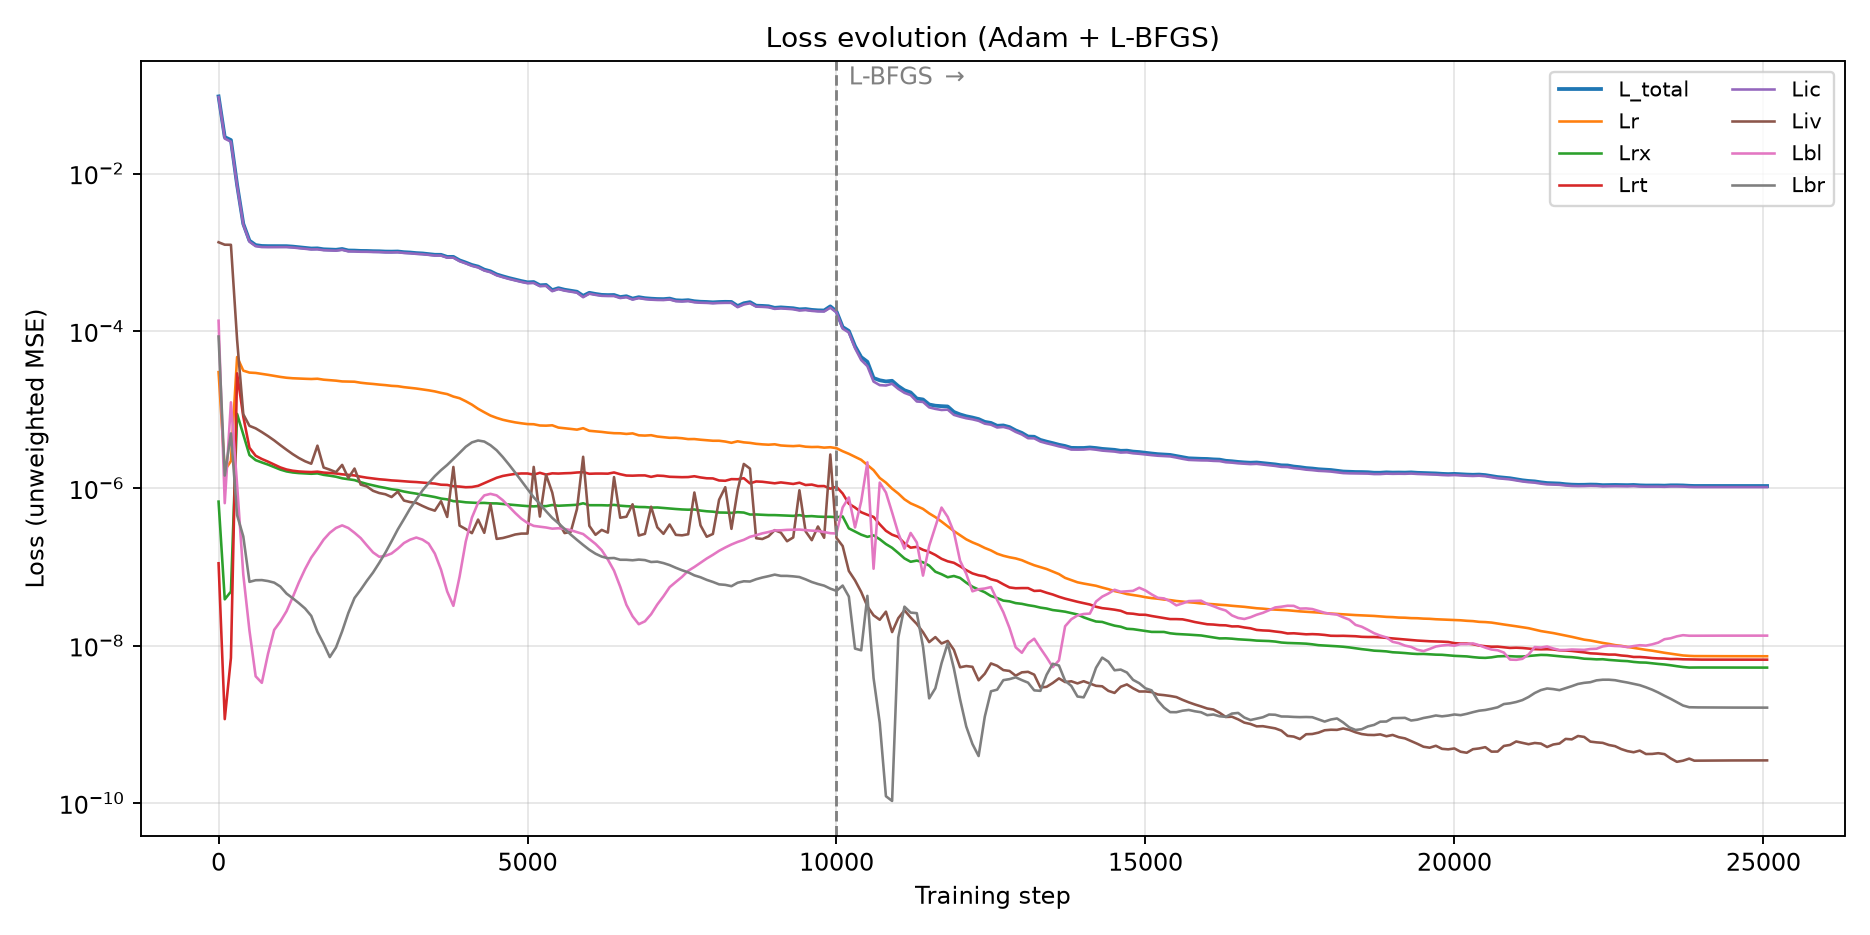
\includegraphics[width=0.80\textwidth]{../outputs/pinn/regge_wheeler_l2_paper/loss.png}
\caption{Faithful-reproduction training histories: total loss
and the seven unweighted components versus training step, with
the Adam--L-BFGS transition at iteration $10{,}000$ marked.
Top: Zerilli. Bottom: Regge--Wheeler.}
\label{fig:repro-loss}
\end{figure}

\paragraph{Isospectral consistency.} The two potentials share
the same QNM spectrum \citep{Chandrasekhar1975}, so a
consistent pipeline must recover compatible $(\omega,\tau)$
from both --- and it does: the M2 damping-time errors agree to
within $0.06$ percentage points ($1.50\%$ versus $1.56\%$),
against a nine-point spread in \citet[Table~3]{Patel2024pinn}.
Having established equivalent behaviour on both potentials,
the remainder of this paper reports on the Zerilli equation.

\FloatBarrier

% --------------------------------------------------------------
\subsection{Enhanced forward PINN}
\label{sec:res-fwd}

How far can the forward field error be driven down at fixed
architecture, and what QNM accuracy does that buy? Starting
from the faithful reproduction of
Sec.~\ref{sec:res-repro}, the enhanced forward PINN doubles the
L-BFGS budget and replaces uniform resampling with the
residual-greedy sampling of Sec.~\ref{sec:fwd-pinn}, all other
settings unchanged. On the FD grid
$x \in [-50,150]\,M$, $t \in [0,50]\,M$ the field-accuracy
metrics are
\begin{equation}
  \mathrm{RMSD} = 8.17\times 10^{-4}, \qquad
  \mathrm{MAD}  = 4.99\times 10^{-4}, \qquad
  \mathrm{RL2}  = 5.79\times 10^{-3},
  \label{eq:fwd-metrics}
\end{equation}
where $\mathrm{RMSD}$ and $\mathrm{MAD}$ are the root-mean-square
and mean-absolute differences $\Phi_\theta - \Phi_{\mathrm{FD}}$ in
absolute units (peak $|\Phi| \approx 0.7$ on the domain), and
$\mathrm{RL2}$ is their relative $L^2$ norm.
This $\mathrm{RL2} = 0.58\%$ is a factor of $\sim\!50$ smaller
than the $\mathrm{RL2} = 28.06\%$ of
\citet[Table~2, Zerilli row]{Patel2024pinn} and a further
factor of $\sim\!2.2$ below the reproduction; the MAD
improvement is $5.0\times 10^{-4}$ versus their
$1.82\times 10^{-2}$, a factor of $\sim\!36$. Field accuracy
at the snapshot times, the global pointwise error, and the
per-component loss history are shown in
Figs.~\ref{fig:fwd-field}--\ref{fig:fwd-loss}.

\begin{figure}[!htbp]
\centering
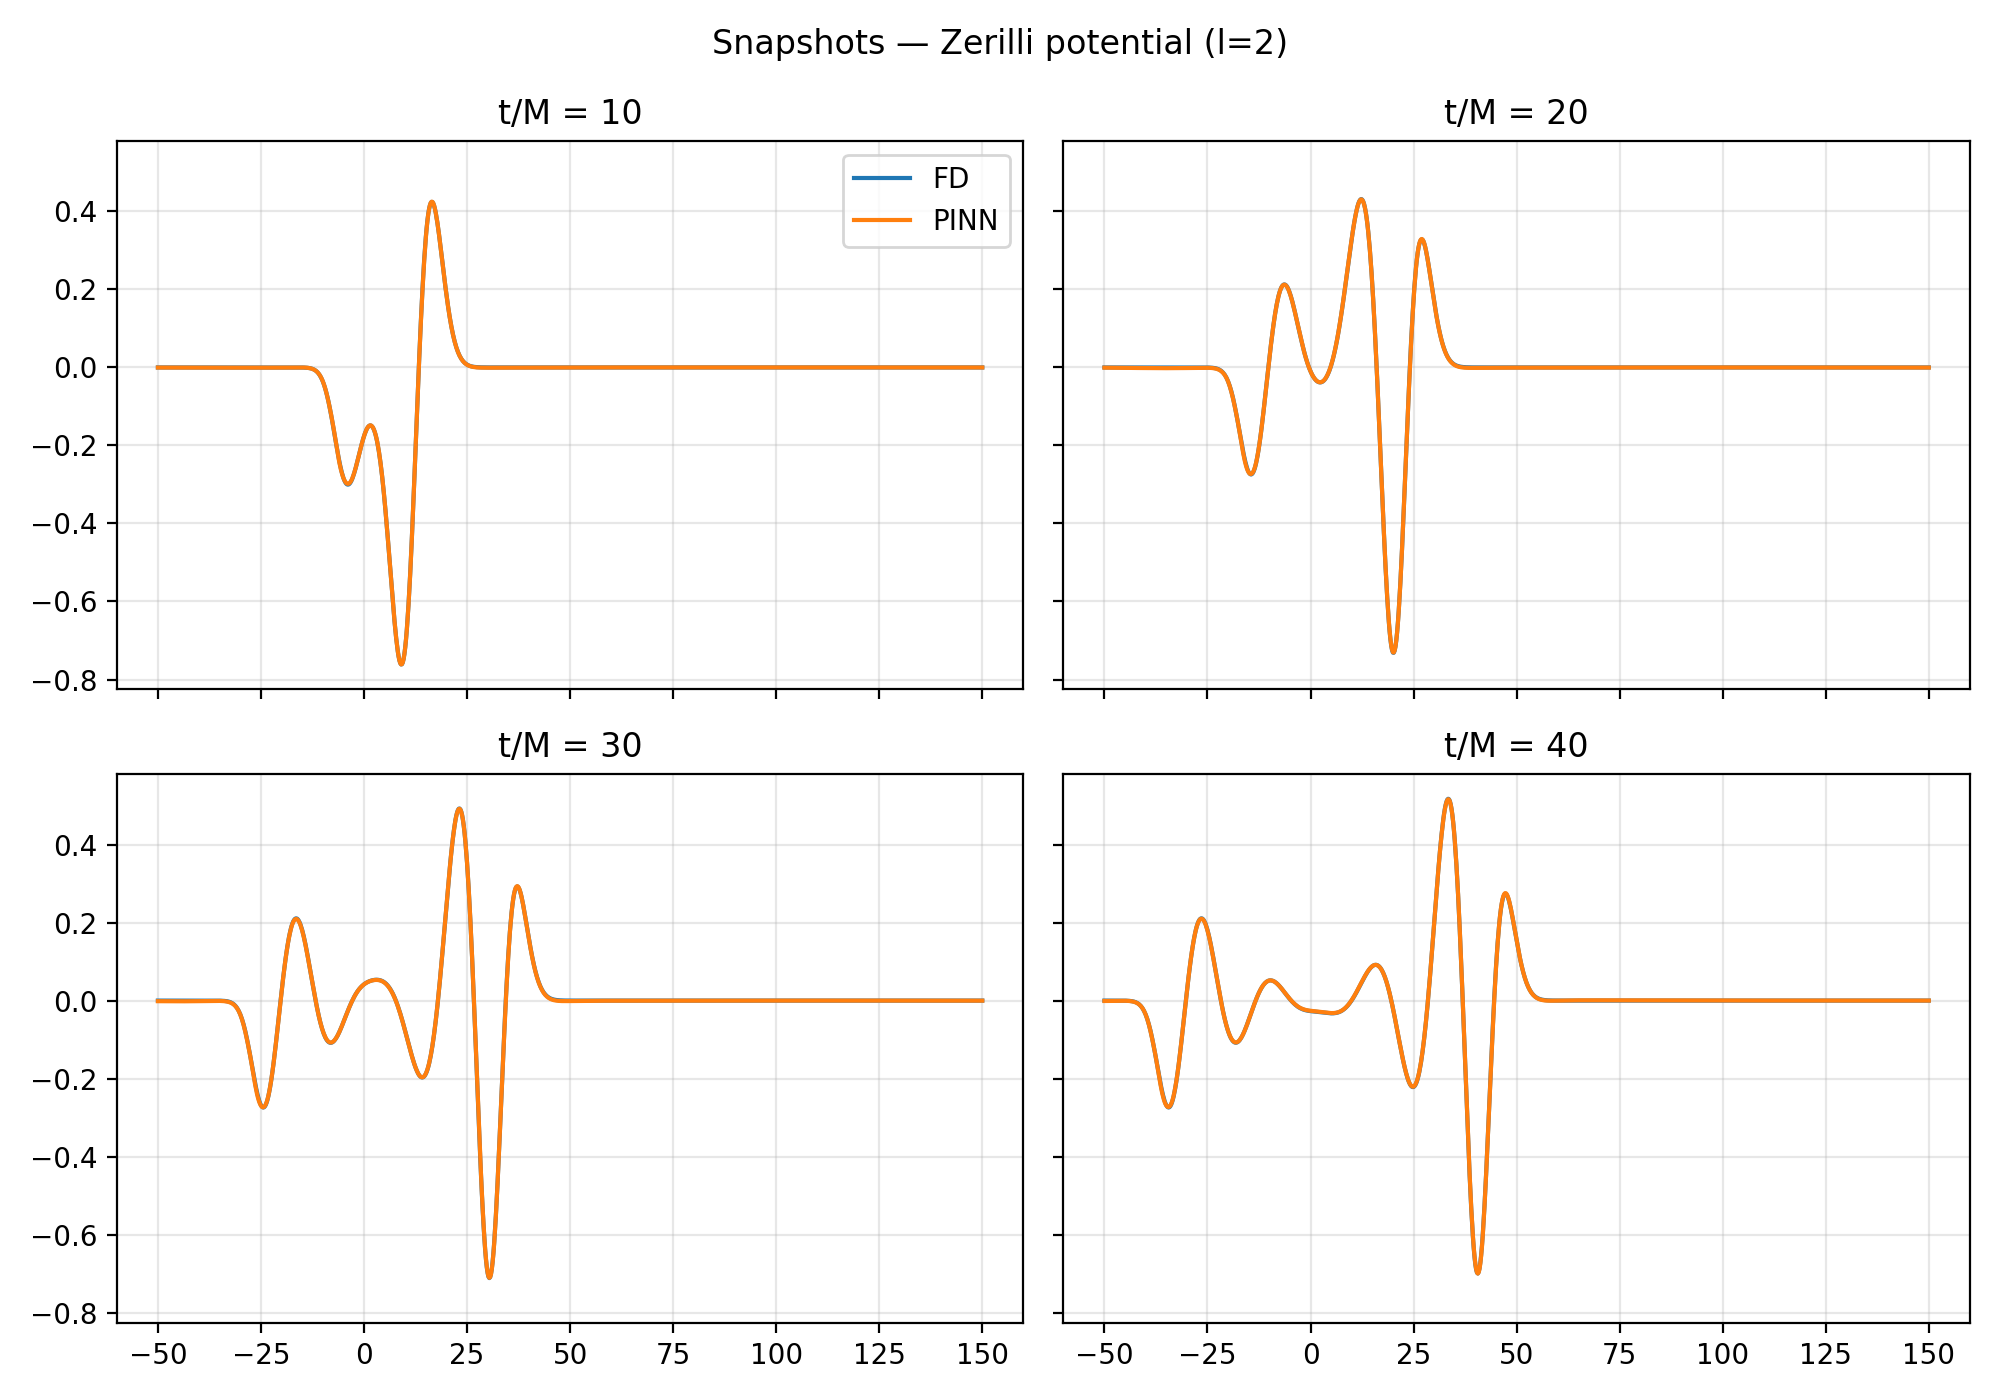
\includegraphics[width=0.82\textwidth]{../outputs/pinn/zerilli_l2_greedy_f03_lbfgs30k/snapshots.png}\\[0.4em]
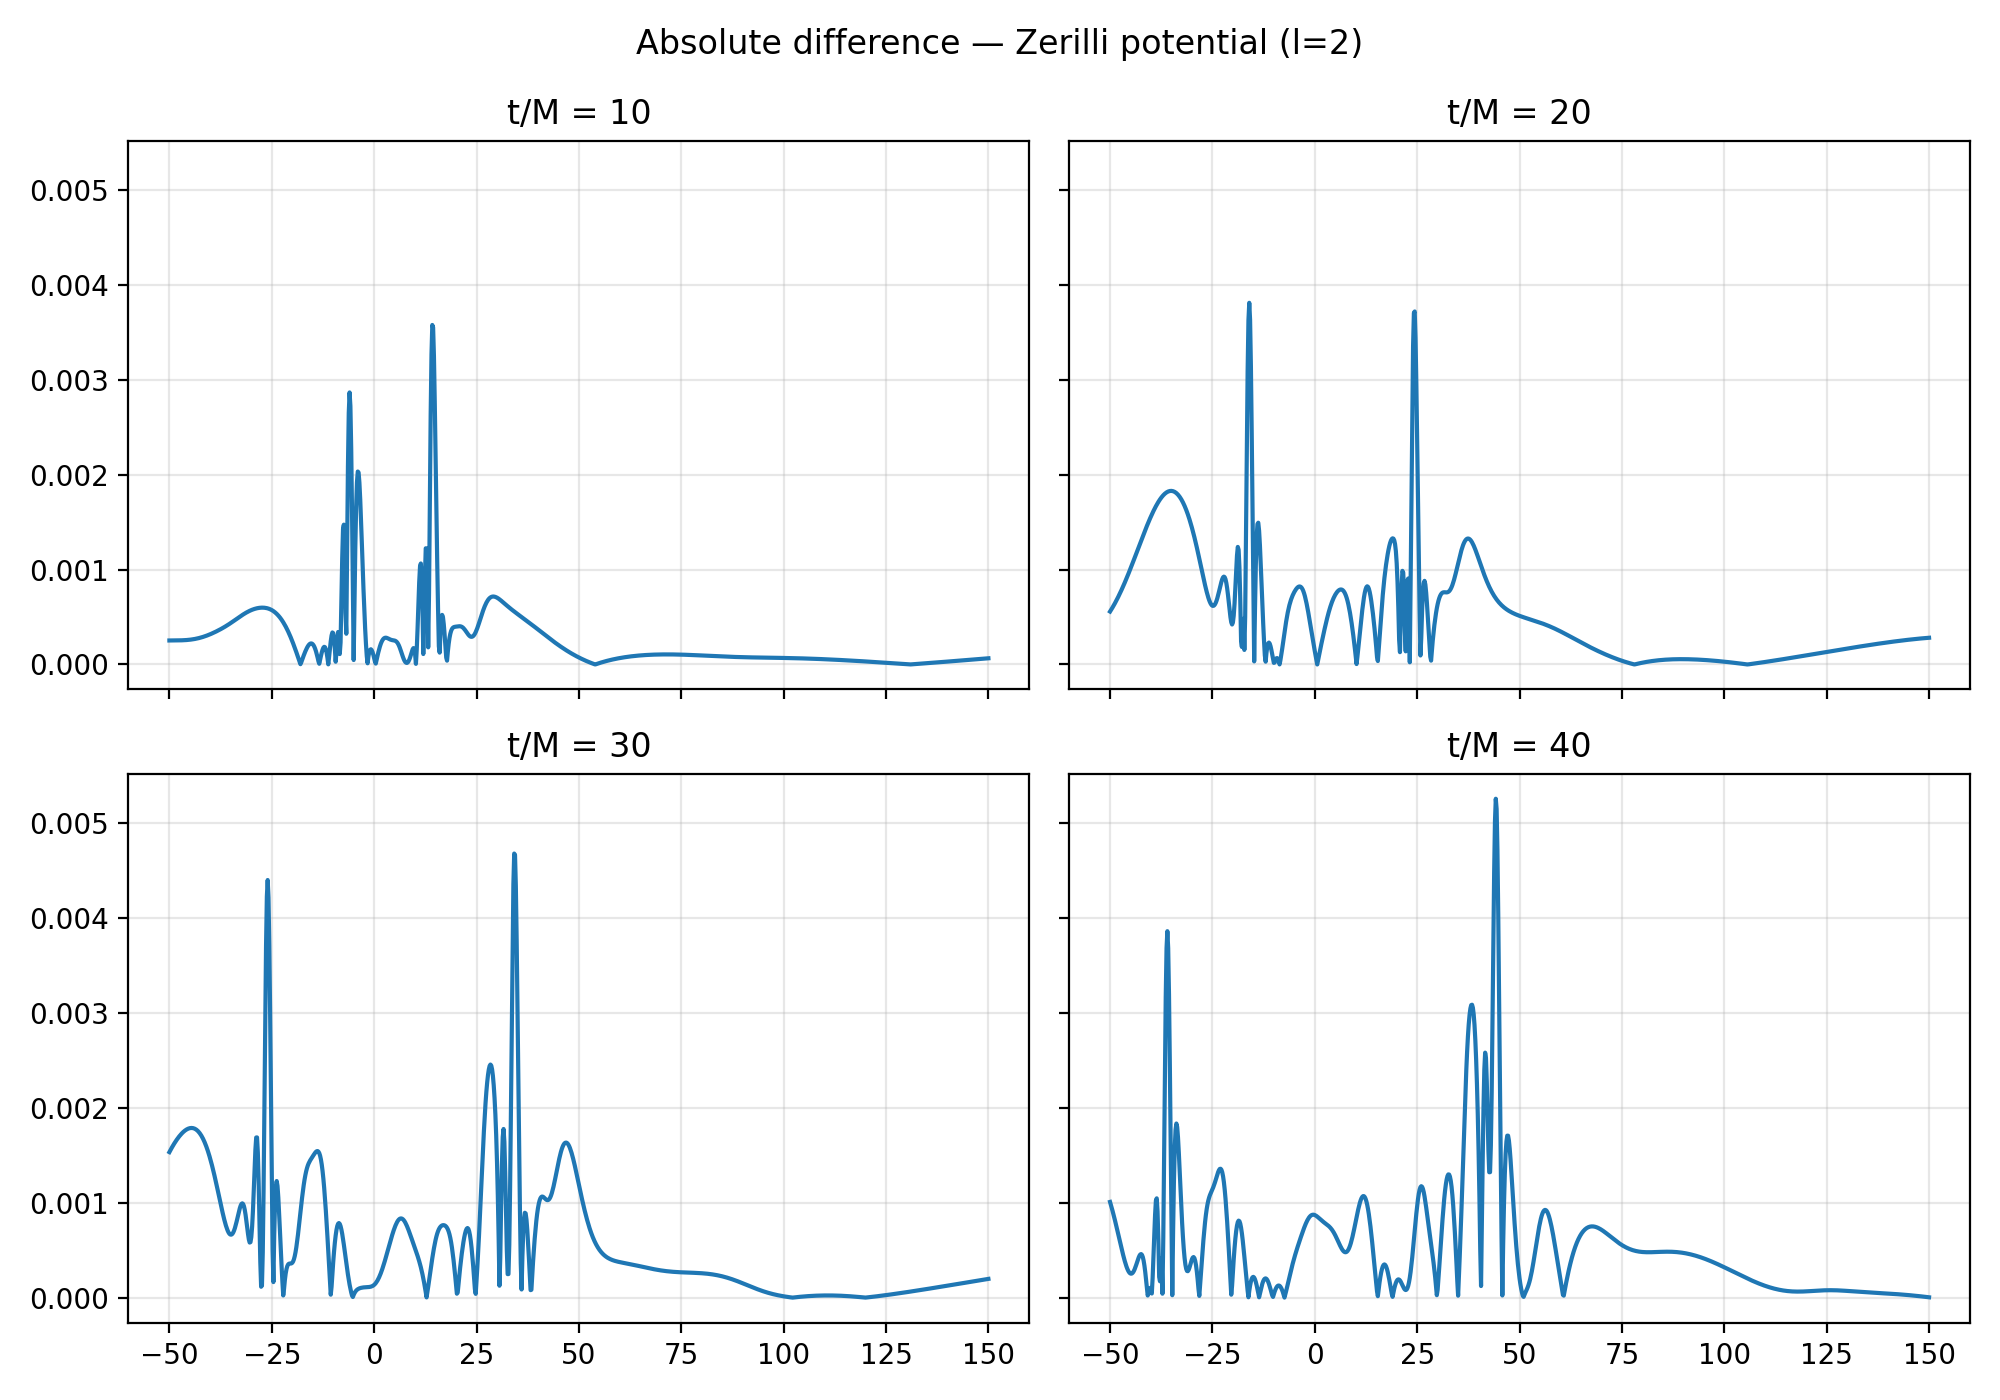
\includegraphics[width=0.82\textwidth]{../outputs/pinn/zerilli_l2_greedy_f03_lbfgs30k/abs_diff_snapshots.png}
\caption{Forward PINN versus FD reference at the snapshot times.
Top: snapshots of $\Phi(x,t)$ at four times
$t/M\in\{10,20,30,40\}$ overlaid for the PINN and the FD
reference; the two curves are visually indistinguishable on this
scale. Bottom: pointwise $|\Phi_\theta - \Phi_{\mathrm{FD}}|$
at the same four times, concentrated near the potential barrier
and remaining below $\sim\!5\times 10^{-3}$ throughout.}
\label{fig:fwd-field}
\end{figure}

\begin{figure}[!htbp]
\centering
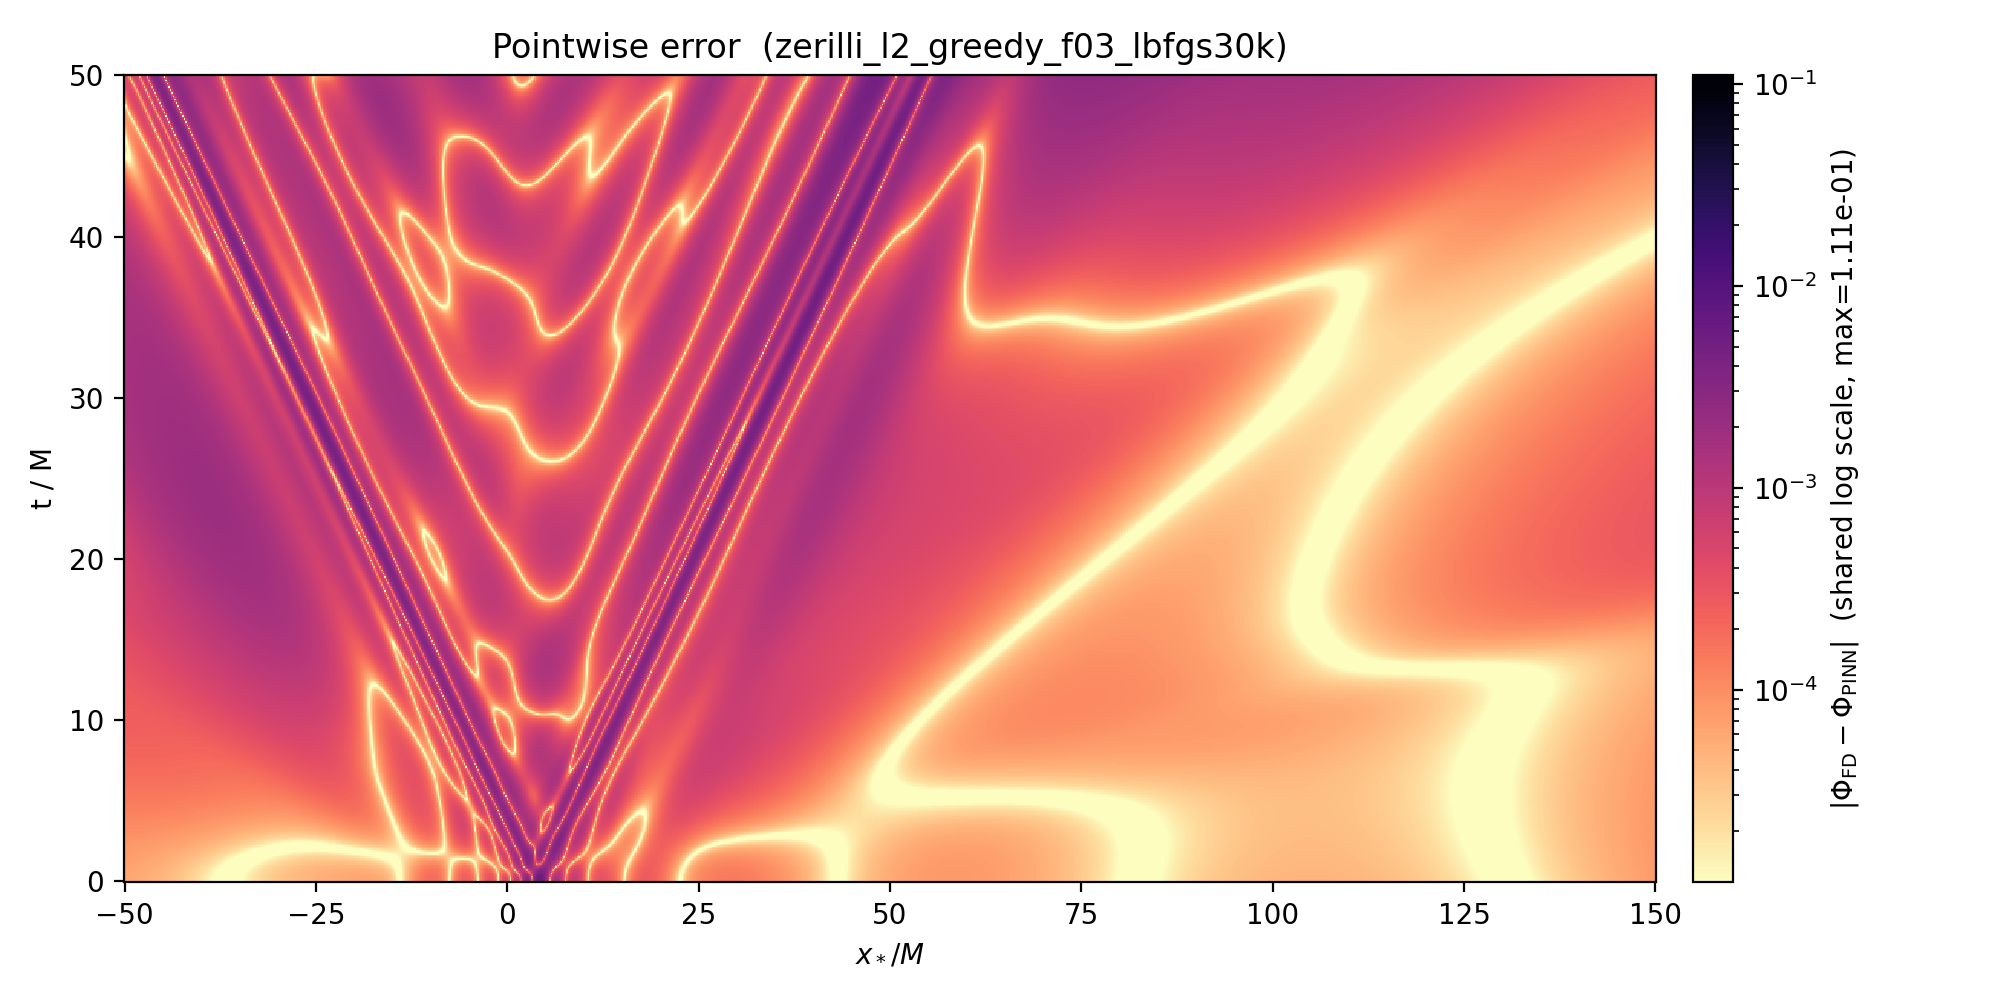
\includegraphics[width=0.92\textwidth]{../outputs/pinn/zerilli_l2_greedy_f03_lbfgs30k/error_heatmap.png}
\caption{Forward PINN global pointwise error. Heatmap of
$|\Phi_\theta - \Phi_{\mathrm{FD}}|$ on the full training domain
$x\in[-50,150]\,M$, $t\in[0,50]\,M$, confirming that the snapshot-time
bound of Fig.~\ref{fig:fwd-field} holds globally.}
\label{fig:fwd-heatmap}
\end{figure}

\begin{figure}[!htbp]
\centering
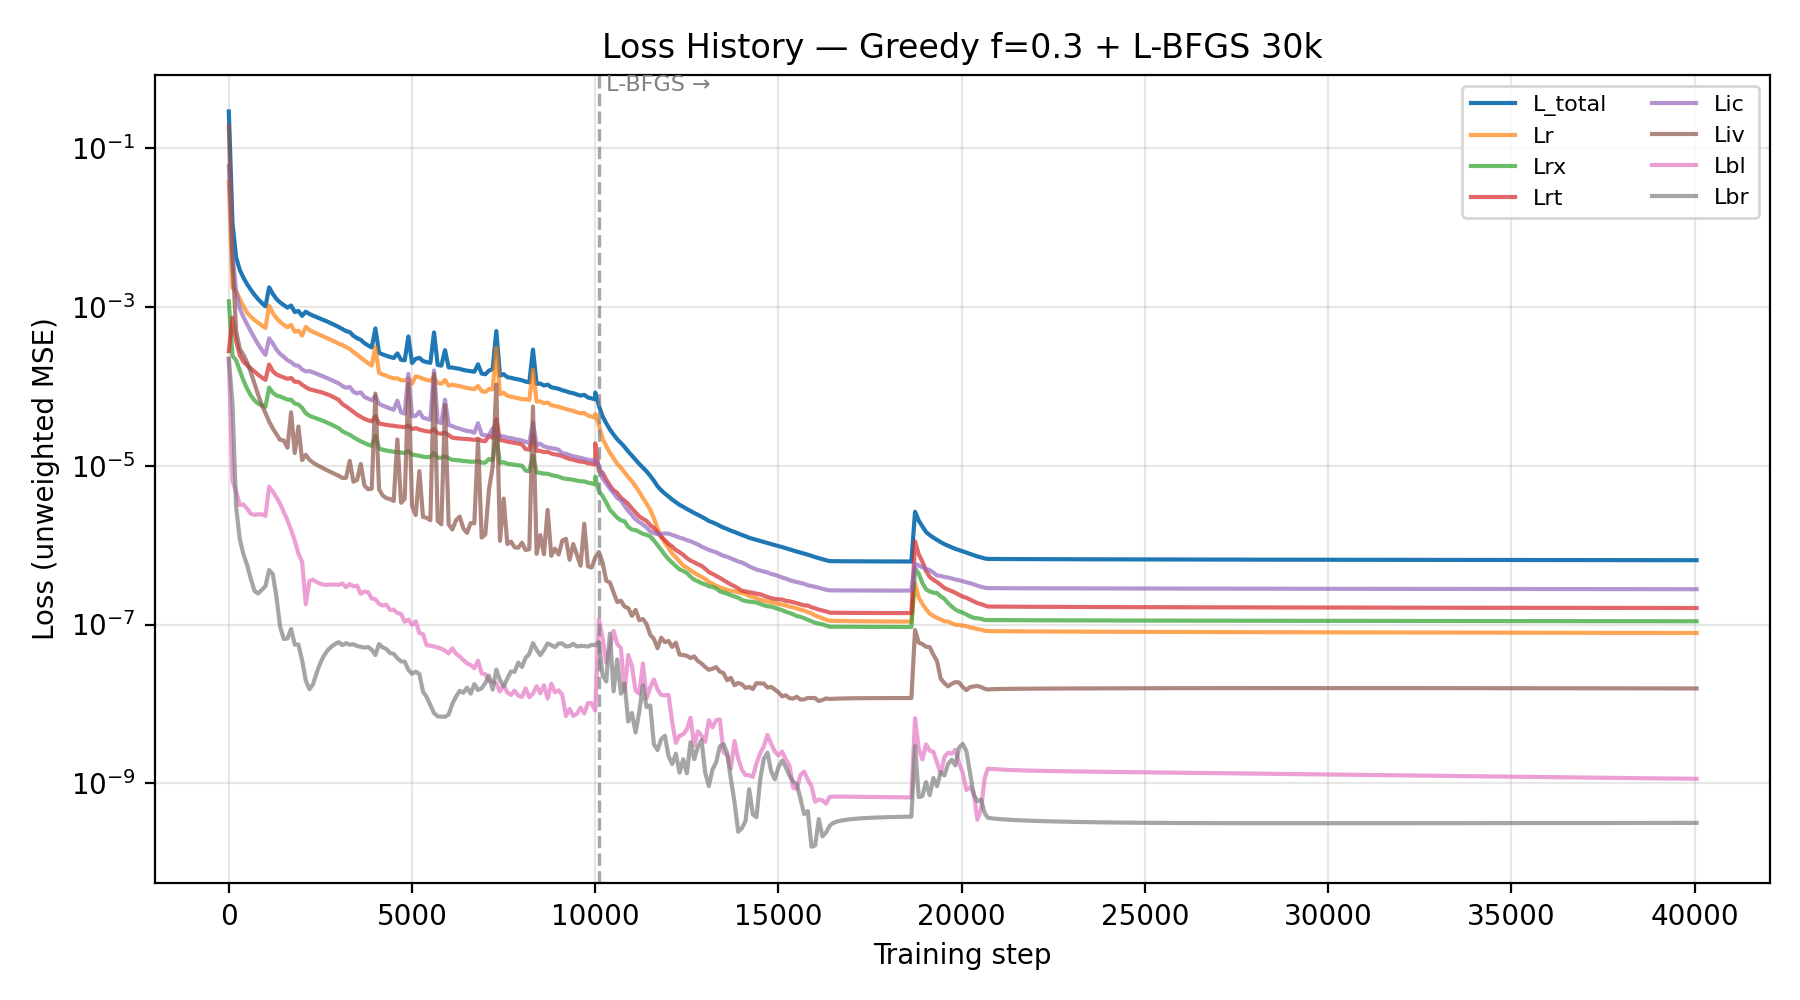
\includegraphics[width=0.85\textwidth]{../outputs/pinn/zerilli_l2_greedy_f03_lbfgs30k/loss.png}
\caption{Forward PINN training history. Total loss
$\mathcal{L}_{\mathrm{tot}}$ and the seven weighted components
($\mathcal{L}_{\mathrm{r}}$, $\mathcal{L}_{\mathrm{rx}}$,
$\mathcal{L}_{\mathrm{rt}}$, $\mathcal{L}_{\mathrm{ic}}$,
$\mathcal{L}_{\mathrm{iv}}$, $\mathcal{L}_{\mathrm{bl}}$,
$\mathcal{L}_{\mathrm{br}}$, weights as in
Sec.~\ref{sec:fwd-pinn}) versus iteration on a log--log axis. The
vertical marker at iteration $10{,}000$ separates the Adam phase
from the L-BFGS phase. The PDE-residual term
$\mathcal{L}_{\mathrm{r}}$ dominates throughout, with the IC and BC
terms below it by one to two orders of magnitude.}
\label{fig:fwd-loss}
\end{figure}

We apply the five extraction methods of Sec.~\ref{sec:qnm-methods}
to the time series $\Phi_\theta(\xq=10\,M,t)$ from the converged
forward PINN. The extracted ringdown, with its single-mode template
overlay, is shown in Fig.~\ref{fig:fwd-ringdown}; the primary
numbers from each method are collected in
Table~\ref{tab:fwd-qnm}, and the plateau diagnostics that justify
the M4 and M5 estimates are shown in Figs.~\ref{fig:fwd-plateau-m4} and~\ref{fig:fwd-plateau-m5}.

\begin{figure}[!htbp]
\centering
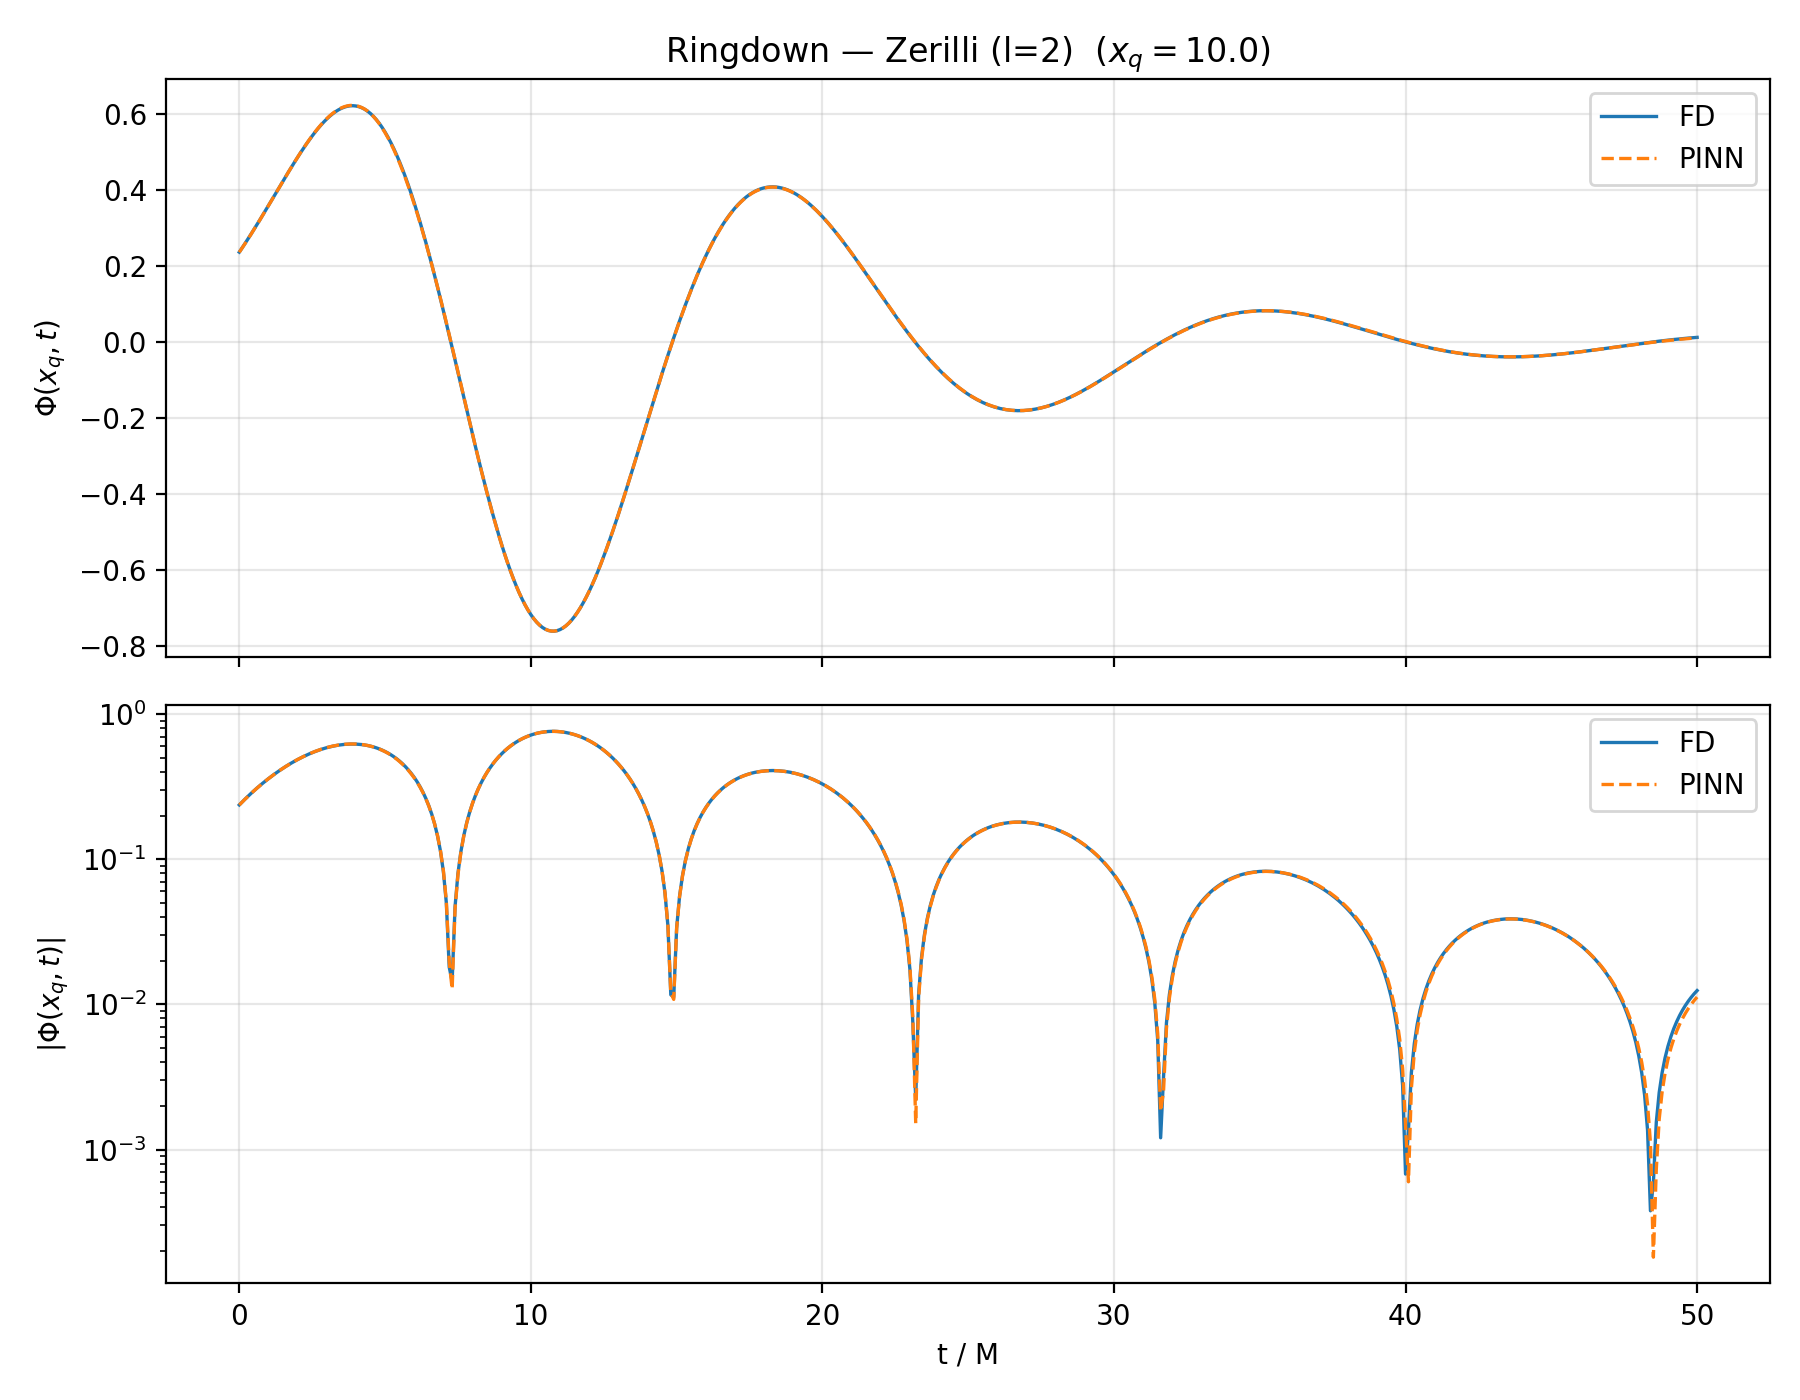
\includegraphics[width=0.85\textwidth]{../outputs/pinn/zerilli_l2_greedy_f03_lbfgs30k/ringdown_overlay.png}\\[0.6em]
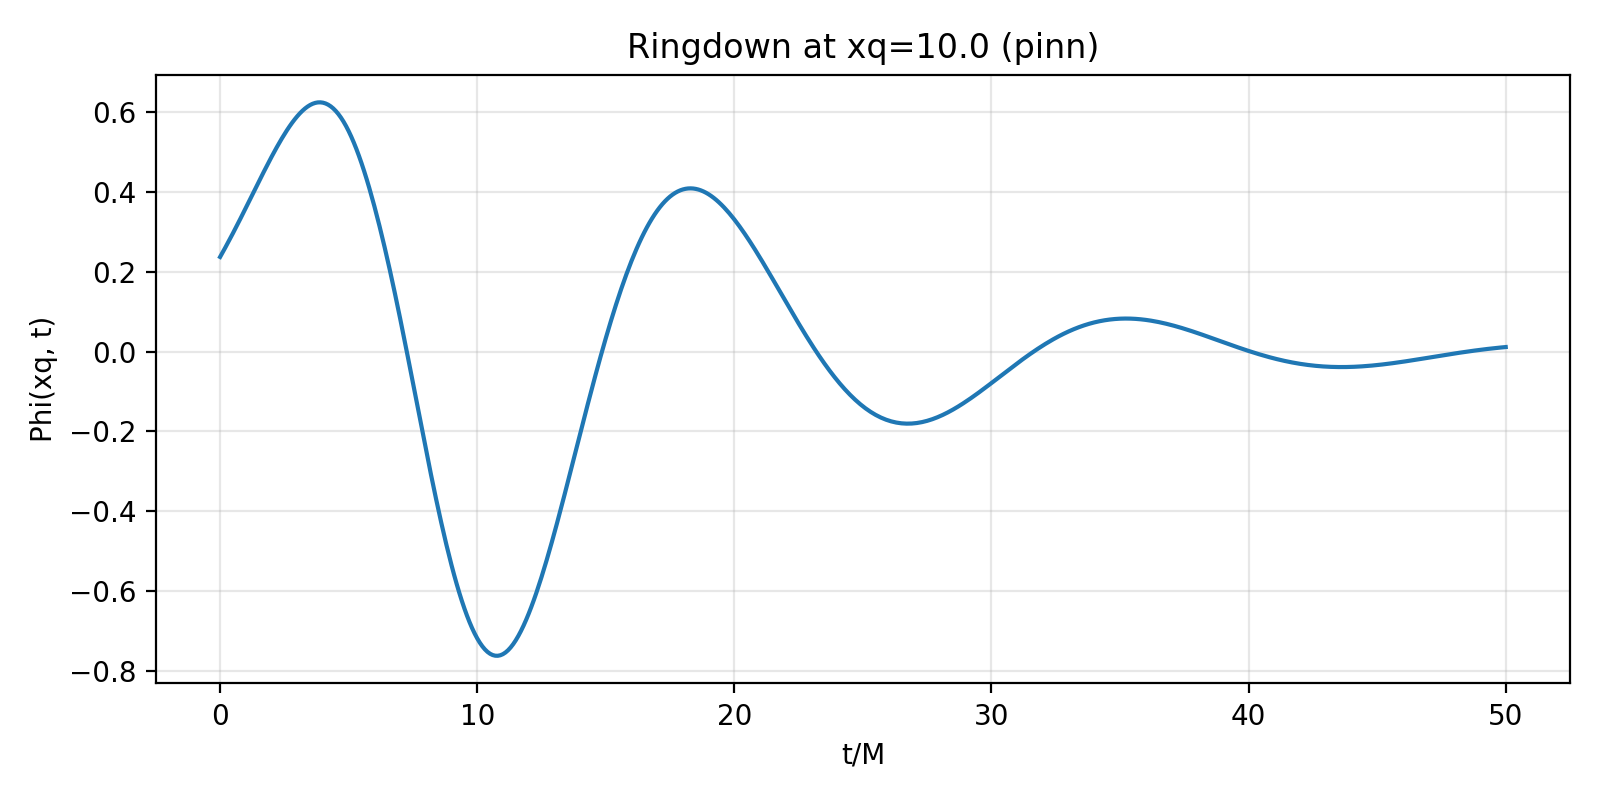
\includegraphics[width=0.85\textwidth]{../outputs/qnm/zerilli_l2_greedy_f03_lbfgs30k/pinn_ringdown.png}
\caption{Forward PINN ringdown at $\xq = 10\,M$. Top two panels:
$\Phi_\theta(\xq,t)$ from the forward PINN overlaid on the FD
reference on linear (upper) and logarithmic (lower) vertical
scales, showing the prompt burst followed by the
exponentially-damped sinusoidal ringdown. Bottom: the same
time series isolated from $\Phi_\theta$, on which the five
extraction methods of Sec.~\ref{sec:qnm-methods} are applied to
produce the entries of Table~\ref{tab:fwd-qnm}.}
\label{fig:fwd-ringdown}
\end{figure}

\begin{table}[!htbp]
\centering
\caption{Forward PINN QNM extraction. Reference values are the
Leaver continued-fraction Schwarzschild $\ell = 2$ fundamental
$M\omega_0 = 0.3737$, $\tau_0/M = 11.241$. ``Wide'' window
denotes $[10,50]\,M$; M2 on plateau denotes M2 evaluated on the
$[t_0^{\min},50]\,M$ window with $t_0^{\min}$ taken as the lower
edge of the M4 plateau. M4 and M5 quote
plateau-mean $\pm$ plateau standard deviation across the
contiguous block of fit windows minimising the combined relative
scatter (Algorithm~\ref{alg:m4} and Sec.~\ref{sec:plateau}).
Bold entries are the primary values under the reporting
convention of Sec.~\ref{sec:reporting}.}
\label{tab:fwd-qnm}
\footnotesize
\setlength{\tabcolsep}{4pt}
\renewcommand{\arraystretch}{1.05}
\begin{tabular}{@{}lccccl@{}}
\toprule
Method & $M\omega$ & $\omega$ err & $\tau/M$ & $\tau$ err & Window or plateau \\
\midrule
M1 (FFT $+$ log-line)        & $0.3712$  & $0.68\%$  & $10.92$ & $2.83\%$ & $[10,\,50]\,M$ \\
M2 (NLS, wide)               & $0.3794$  & $1.54\%$  & $11.464$ & $\mathbf{1.99\%}$ & $[10,\,50]\,M$ \\
M2 (NLS on M4 plateau)       & $0.3749$  & $0.31\%$  & $10.41$ & $7.38\%$ & $[14,\,50]\,M$ \\
M3 (ESPRIT, $K=6$)           & $0.4829$  & $29.2\%$  & $7.84$  & $30.3\%$ & $[10,\,50]\,M$ \\
M4 (1-D plateau)             & $0.37359{\pm}2{\times}10^{-4}$ & $\mathbf{0.029\%}$ & $10.94{\pm}0.02$ & $2.65\%$ & $t_0\in[14,21]M$, $\tend{=}50M$ \\
M5 (2-D plateau)             & $0.3728{\pm}8{\times}10^{-4}$ & $0.23\%$ & $10.80{\pm}0.12$ & $3.91\%$ & $t_0\in[10,16.7]M$, $\tend\in[42,50]M$ \\
\bottomrule
\end{tabular}
\end{table}

\begin{figure}[!htbp]
\centering
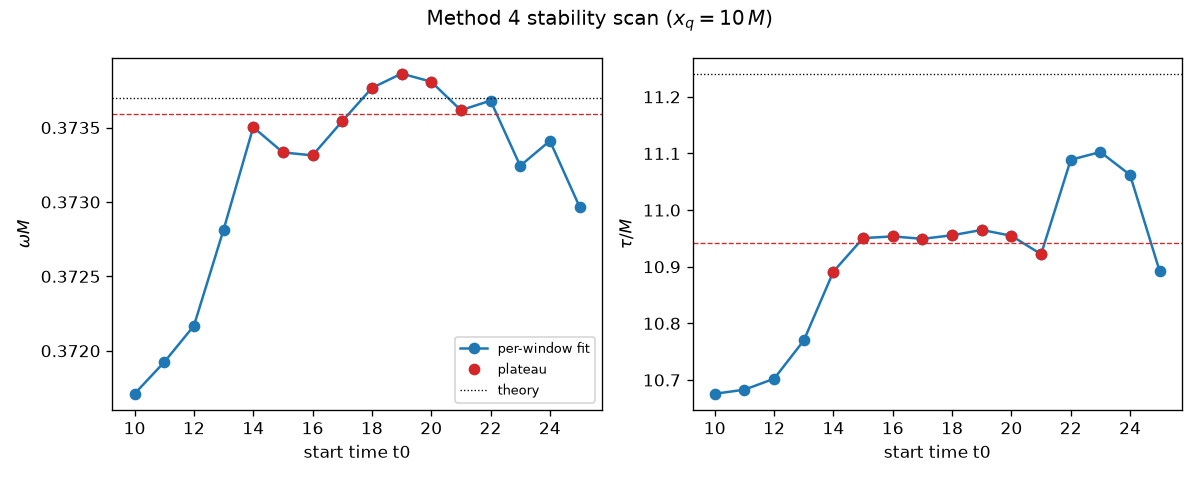
\includegraphics[width=0.95\textwidth]{../outputs/qnm/zerilli_l2_greedy_f03_lbfgs30k/pinn_method4_stability.png}
\caption{M4 plateau diagnostic for the forward PINN.
$(\omega_0,\tau_0)$ as a function of the start time $t_0$ on
$[10,25]\,M$ at fixed $\tend = 50\,M$, with the eight-window
plateau block ($t_0\in[14,21]\,M$) shaded.}
\label{fig:fwd-plateau-m4}
\end{figure}

\begin{figure}[!htbp]
\centering
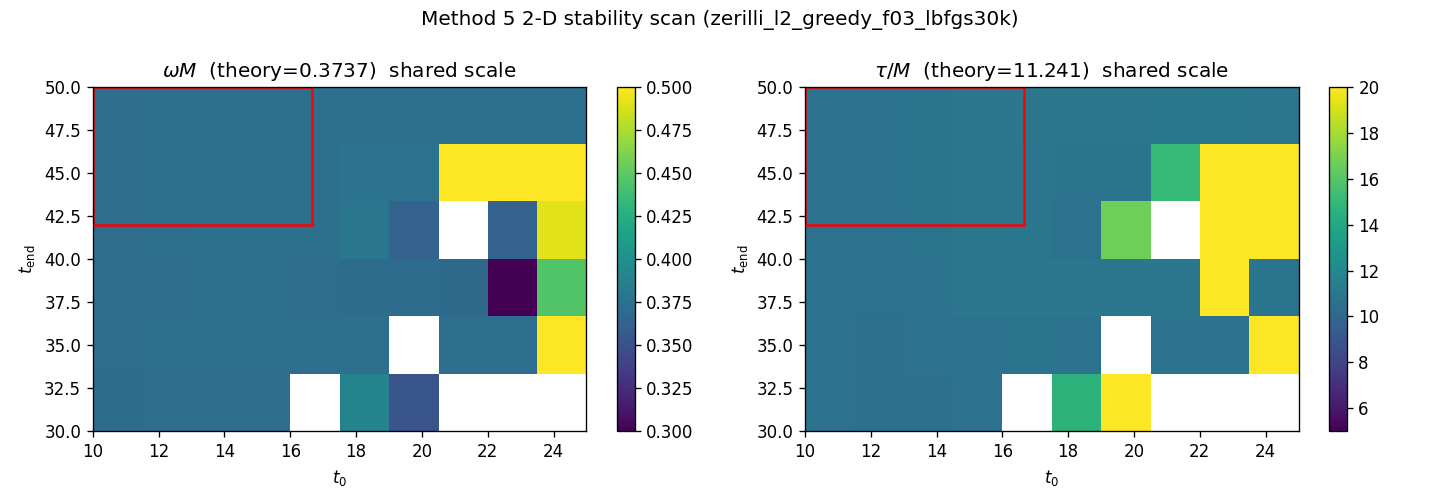
\includegraphics[width=0.85\textwidth,keepaspectratio]{../outputs/qnm/zerilli_l2_greedy_f03_lbfgs30k/pinn_method5_2d_heatmap.png}
\caption{M5 plateau diagnostic for the forward PINN. Heatmap of
the absolute deviation of the M2 estimate from the plateau median
on the $(t_0,\tend)$ grid (capped at $5\%$); the contiguous
$5\times 3$ plateau rectangle is outlined in red. Top:
$\omega_0$. Bottom: $\tau_0$. Annotations report the in-block
relative scatter (the quantity the plateau rule minimises) and
the bias of the plateau mean from the Leaver value.}
\label{fig:fwd-plateau-m5}
\end{figure}

Two points stand out. The M4 plateau estimate reaches
$0.029\%$ in $\omega$, an order of magnitude tighter than any
single-window method, while M2 on the M4 plateau window
sharpens $\omega$ but degrades $\tau$, so $\omega$ and $\tau$
are taken from different estimators under the selection rule of
Sec.~\ref{sec:reporting}.
M3 returns frequencies at machine-precision amplitudes and is
quoted in Appendix~\ref{app:esprit} only.

\paragraph{Error budget.} The two measured contributions to
the frequency error rank as follows: the M4 bias against the
Leaver value is $1.1\times 10^{-4}$ in $M\omega$ ($0.029\%$),
and the fit-window systematic is $\sigma_\omega = 2\times 10^{-4}$
($0.054\%$; a lower bound, Sec.~\ref{sec:plateau}). The
frequency measurement is therefore
window-limited, not field-limited. For the
M4 damping time the ordering reverses: its plateau scatter
$\sigma_\tau/\tau \approx 0.2\%$ sits against a $2.65\%$ bias, so
the M4 $\tau$ is field- and template-limited rather than
window-limited; the Leaver-closest damping time is instead M2 on
the wide window ($1.99\%$), the value reported in
Table~\ref{tab:results-summary}.

\FloatBarrier

% --------------------------------------------------------------
\subsection{Hybrid coarse-FD + neural-residual surrogate}
\label{sec:res-hyb}

The final model asks how much of the fine solver's
accuracy can be recovered from a classical solve at $1/64$ of
its cost. The hybrid surrogate of Sec.~\ref{sec:hyb-method}
keeps a coarse-grid FD solve to carry the wave propagation and
asks the
network only
for the pointwise residual against the fine-grid solution of
the same problem. It is evaluated on the canonical draw
$(M,x_{0},\sigma) = (1,4,5)$ and on a $100$-BH in-distribution
Sobol test set (drawn from the hybrid's own training box,
Sec.~\ref{sec:hyb-method}), at coarsening factor $k = 4$ with
the label-free Richardson training target of
Eqs.~\eqref{eq:hyb-richardson}--\eqref{eq:hyb-residual};
extraction is at the common observer $\xq = 10\,M$ shared with
the PINNs, over the model's full $[10,100]\,M$ evolution. The $k = 4$ prior is deliberately weak ($4.93\%$ relative
$L^{2}$ on the canonical draw), leaving a large but
spatially-localised dispersion error for the gated network to
repair.

\paragraph{Field accuracy on the canonical BH.} The hybrid
reproduces the fine FD reference with gridwise
$\mathrm{RMSD} = 6.28\times 10^{-4}$, against
$6.95\times 10^{-3}$ for the quintic-spline upsample of the
coarse solve alone (henceforth the \emph{coarse-up baseline}):
the gated residual suppresses
the coarse-prior discretisation error by a factor of $11.1$
(equivalently $0.445\%$ versus $4.93\%$ in relative $L^{2}$).
The residual is concentrated on the outgoing wavefronts where
the coarse prior dephases (Fig.~\ref{fig:hyb-snapshots}); the
global error maps (Figs.~\ref{fig:hyb-heatmap}
and~\ref{fig:hyb-heatmap-base}) show the hybrid suppressing
the baseline's dispersion characteristics by roughly an order
of magnitude while leaving the smooth interior and causal
exterior at the prior --- the correction lands exactly where
the gate directs it.

\begin{figure}[!htbp]
\centering
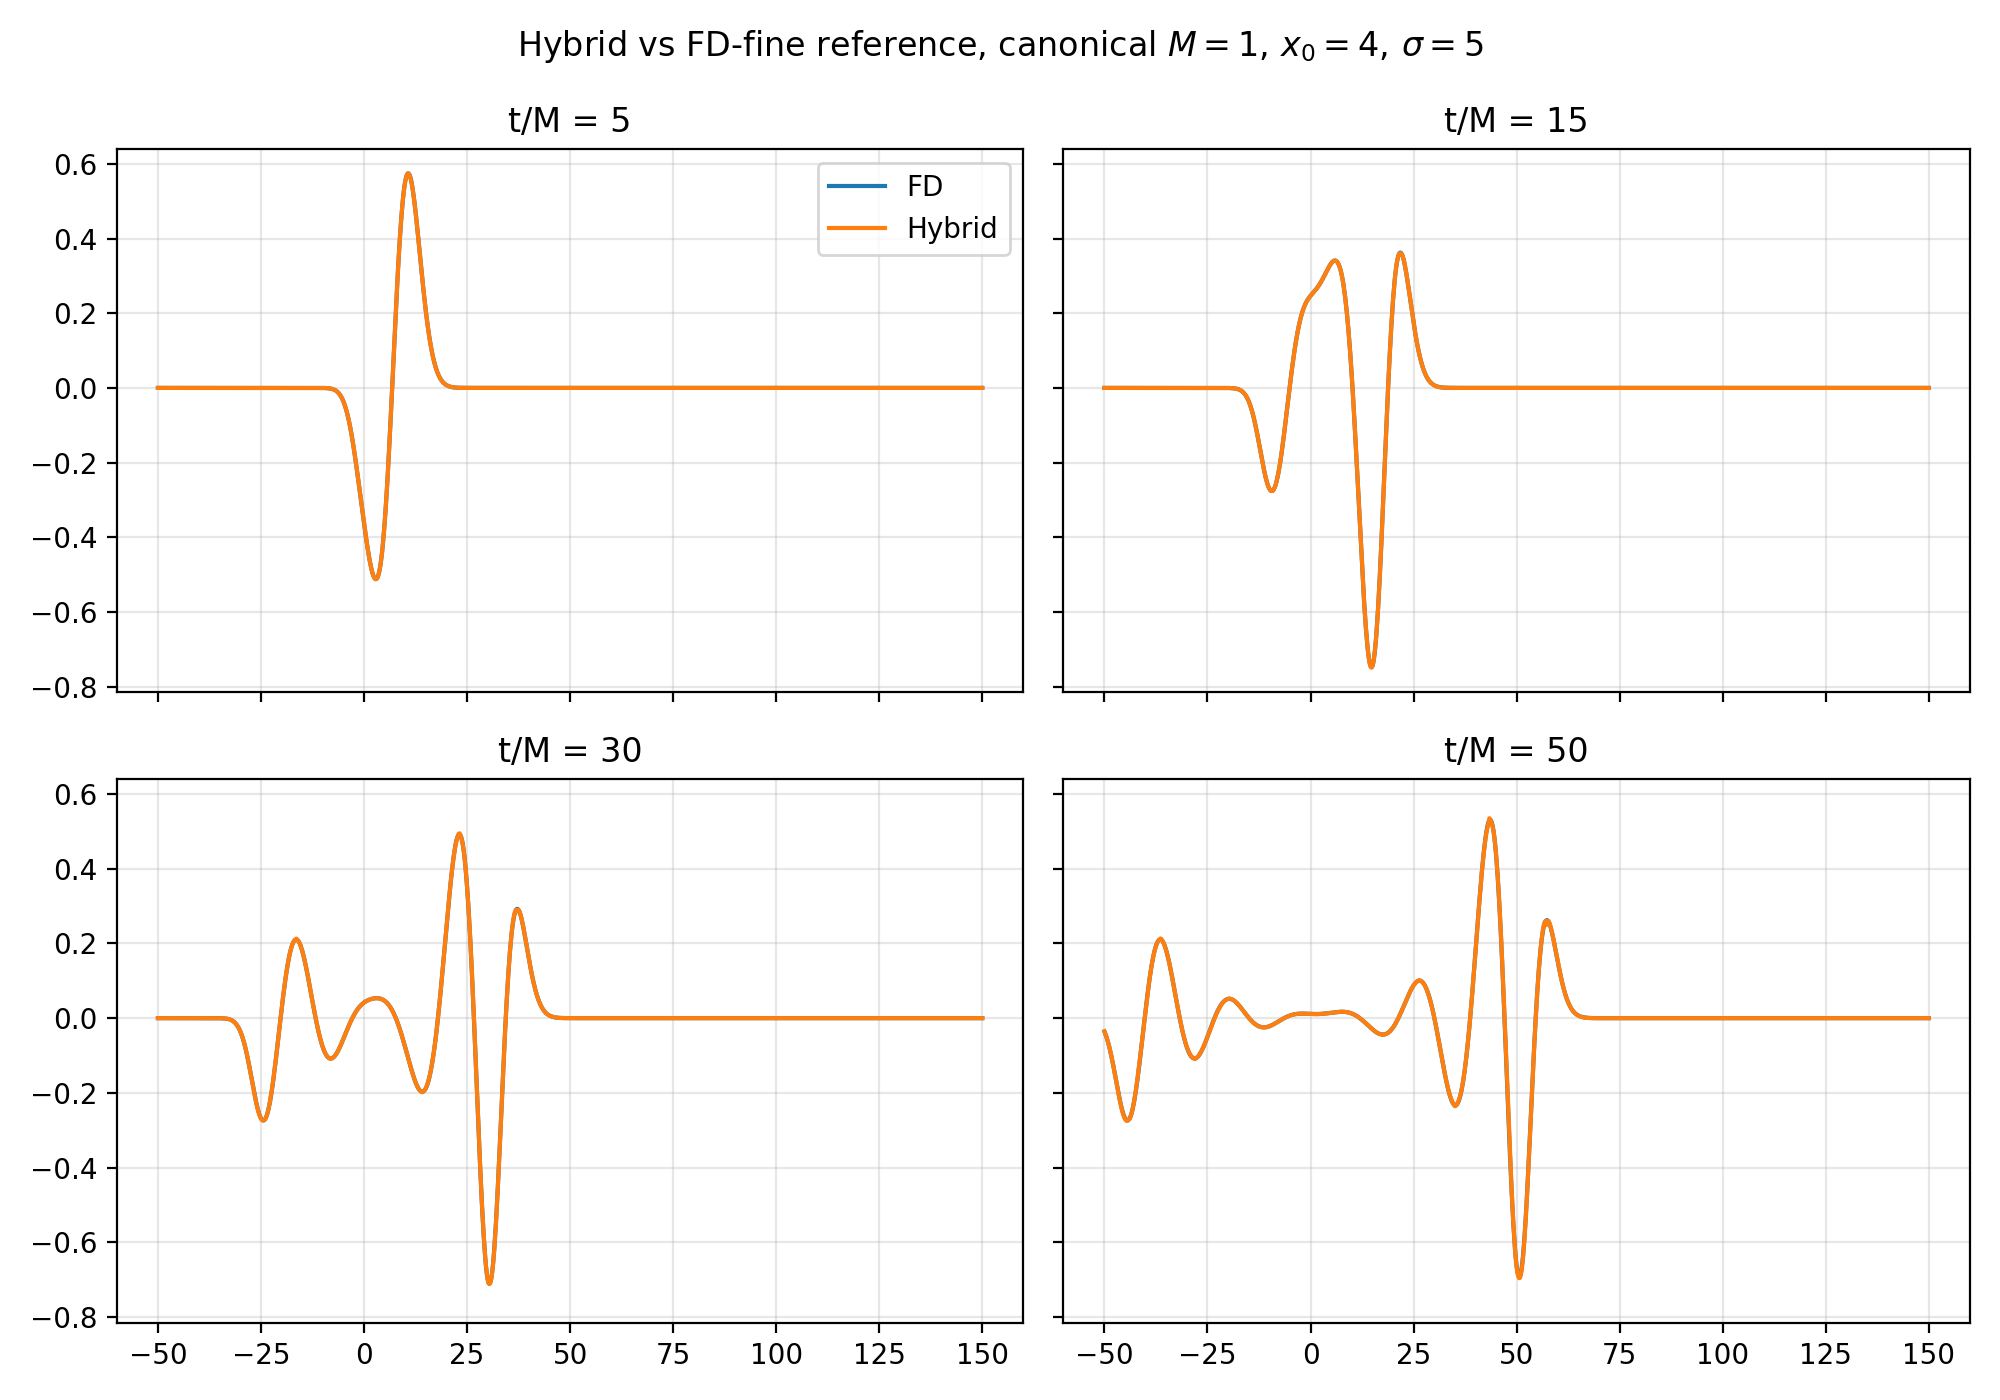
\includegraphics[width=0.82\textwidth]{../outputs/hybrid/fno_sw_gate_s1em3/figs/hybrid_snapshots.png}\\[0.4em]
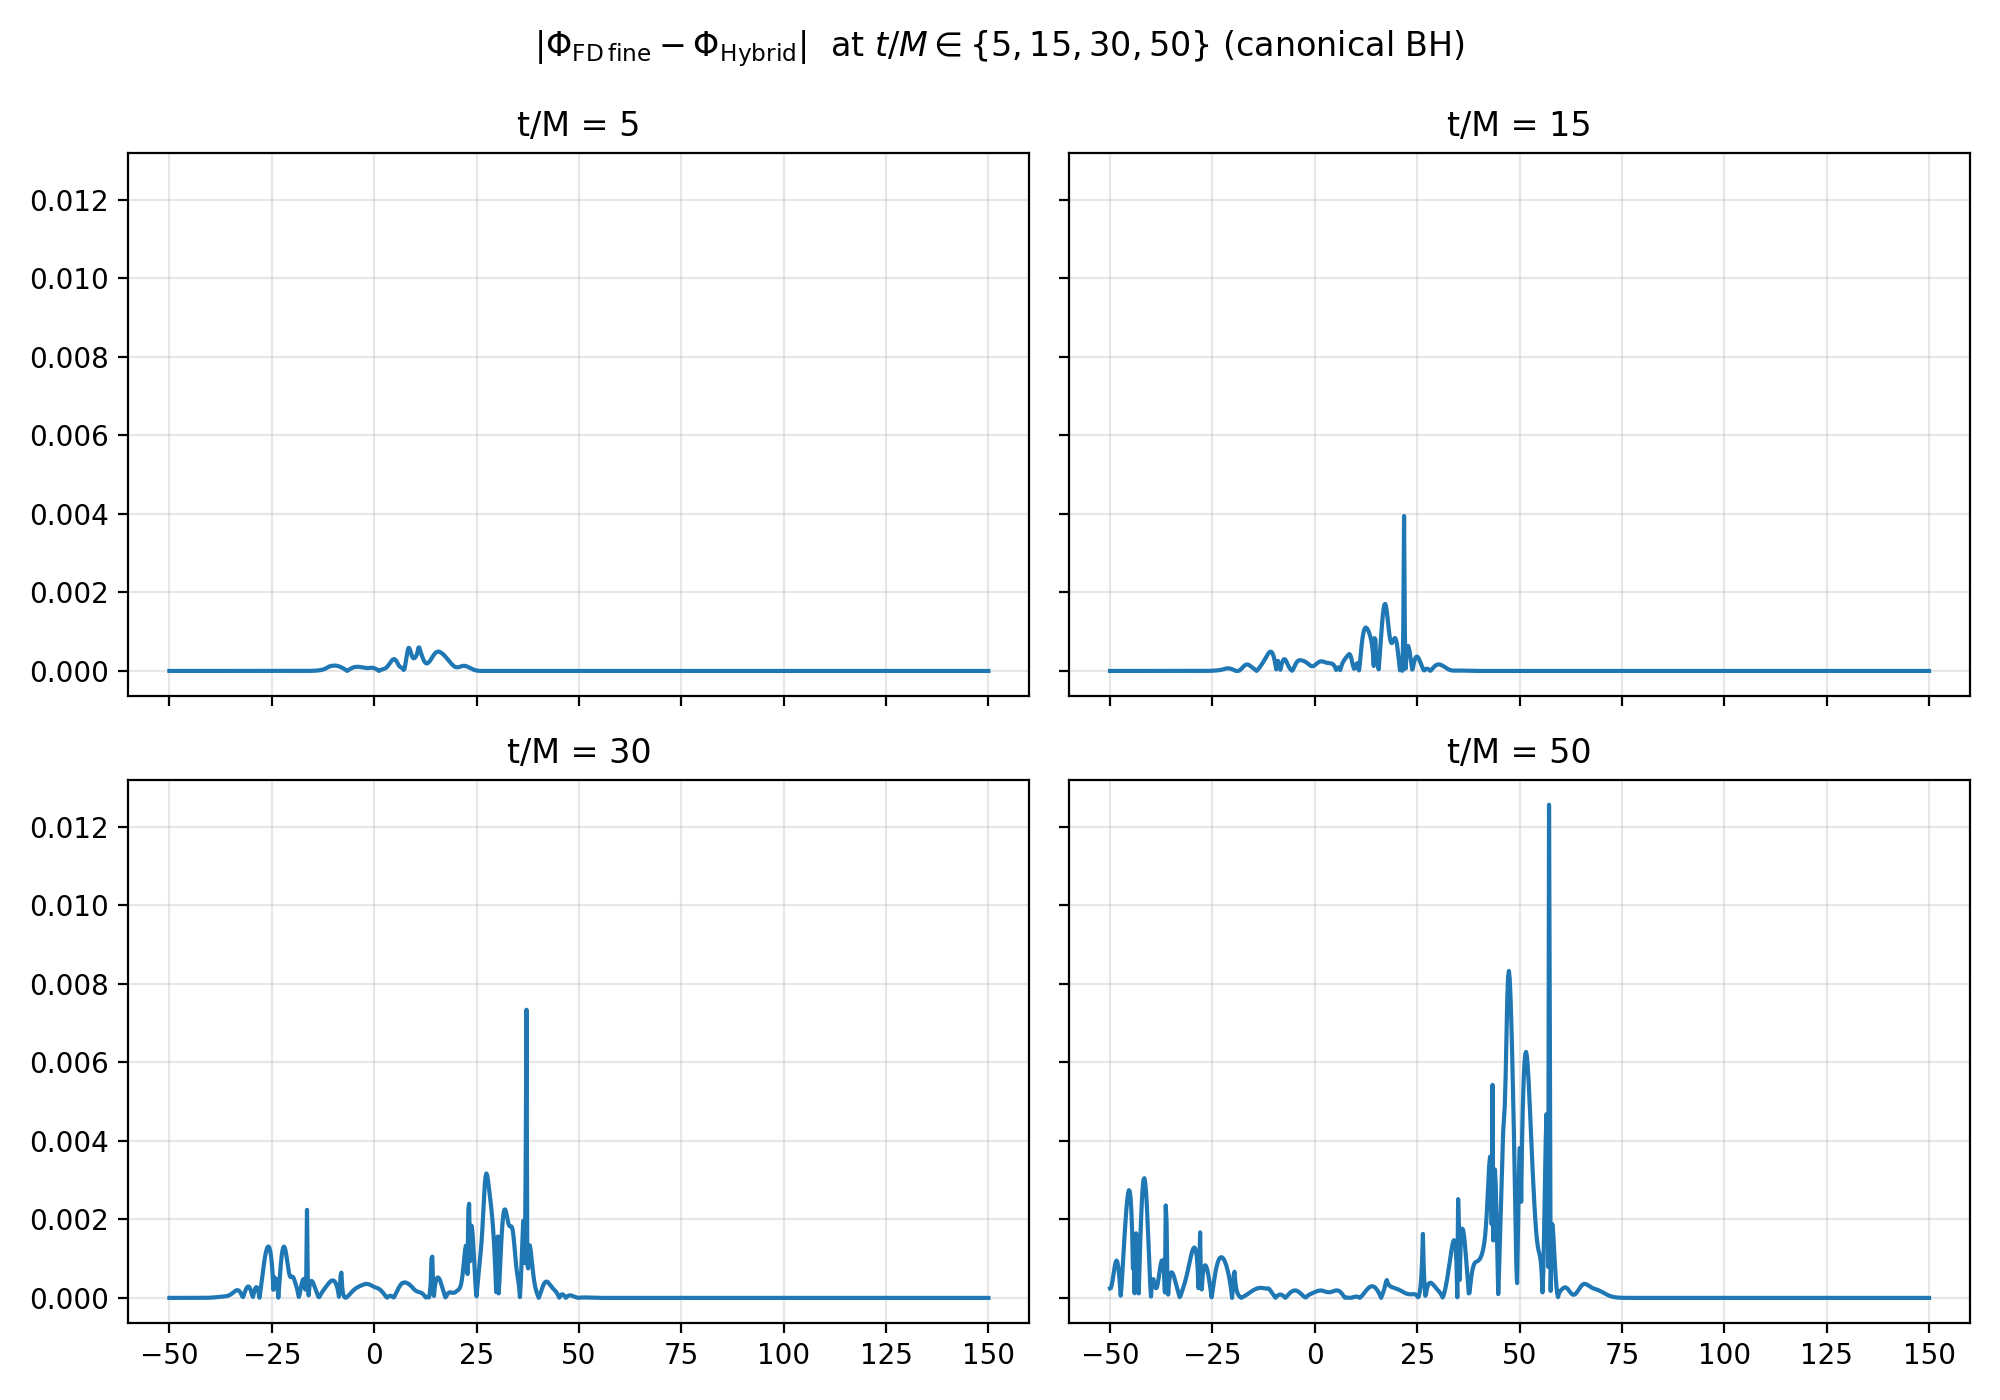
\includegraphics[width=0.82\textwidth]{../outputs/hybrid/fno_sw_gate_s1em3/figs/hybrid_abs_diff_snapshots.png}
\caption{Hybrid prediction versus fine FD reference on the
canonical BH at four snapshot times. Top: $\Phi(x,t)$ at
$t/M \in \{5, 15, 30, 50\}$, with the fine FD reference (blue)
and the hybrid prediction (orange) overlaid; the two curves
are visually indistinguishable on this scale. Bottom: pointwise
$|\Phi^{\mathrm{f}} - \Phi^{\mathrm{hyb}}|$ at the same four
times, concentrated on the outgoing wavefronts and near-zero
across the smooth interior and the causal exterior.}
\label{fig:hyb-snapshots}
\end{figure}

\begin{figure}[!htbp]
\centering
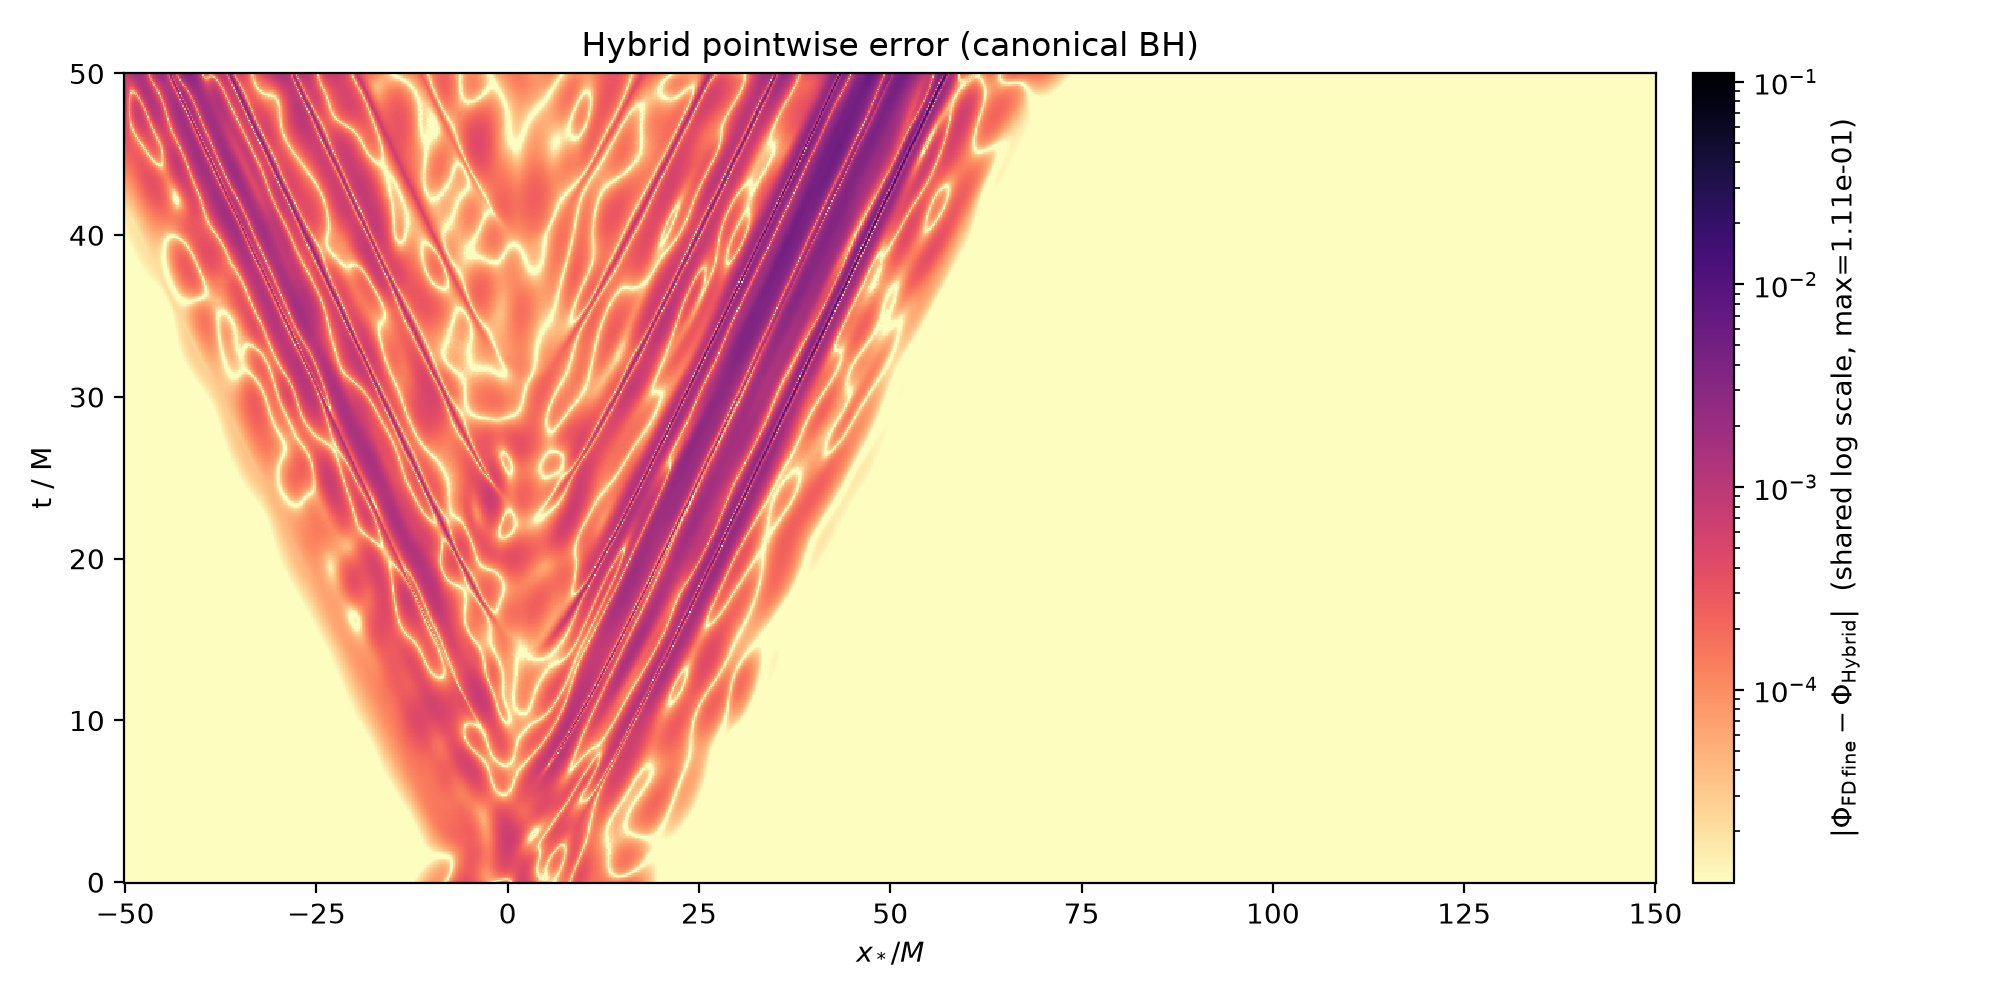
\includegraphics[width=0.92\textwidth]{../outputs/hybrid/fno_sw_gate_s1em3/figs/hybrid_pointwise_error.png}
\caption{Hybrid surrogate global pointwise error on the
canonical BH. Heatmap of
$|\Phi^{\mathrm{f}} - \Phi^{\mathrm{hyb}}|$ on
$x \in [-50, 150]\,M$, $t \in [0, 50]\,M$ (the full hybrid
training and evaluation window), plotted on a
logarithmic $\mathrm{magma\_r}$ colour
scale. The residual structure is confined by the
gradient gate to the prompt-burst region $t \lesssim 5\,M$ and
the outgoing wavefronts; the smooth interior and causal
exterior are left at the prior. Compare with the
coarse-up baseline error on the same
colour scale in Fig.~\ref{fig:hyb-heatmap-base}.}
\label{fig:hyb-heatmap}
\end{figure}

\begin{figure}[!htbp]
\centering
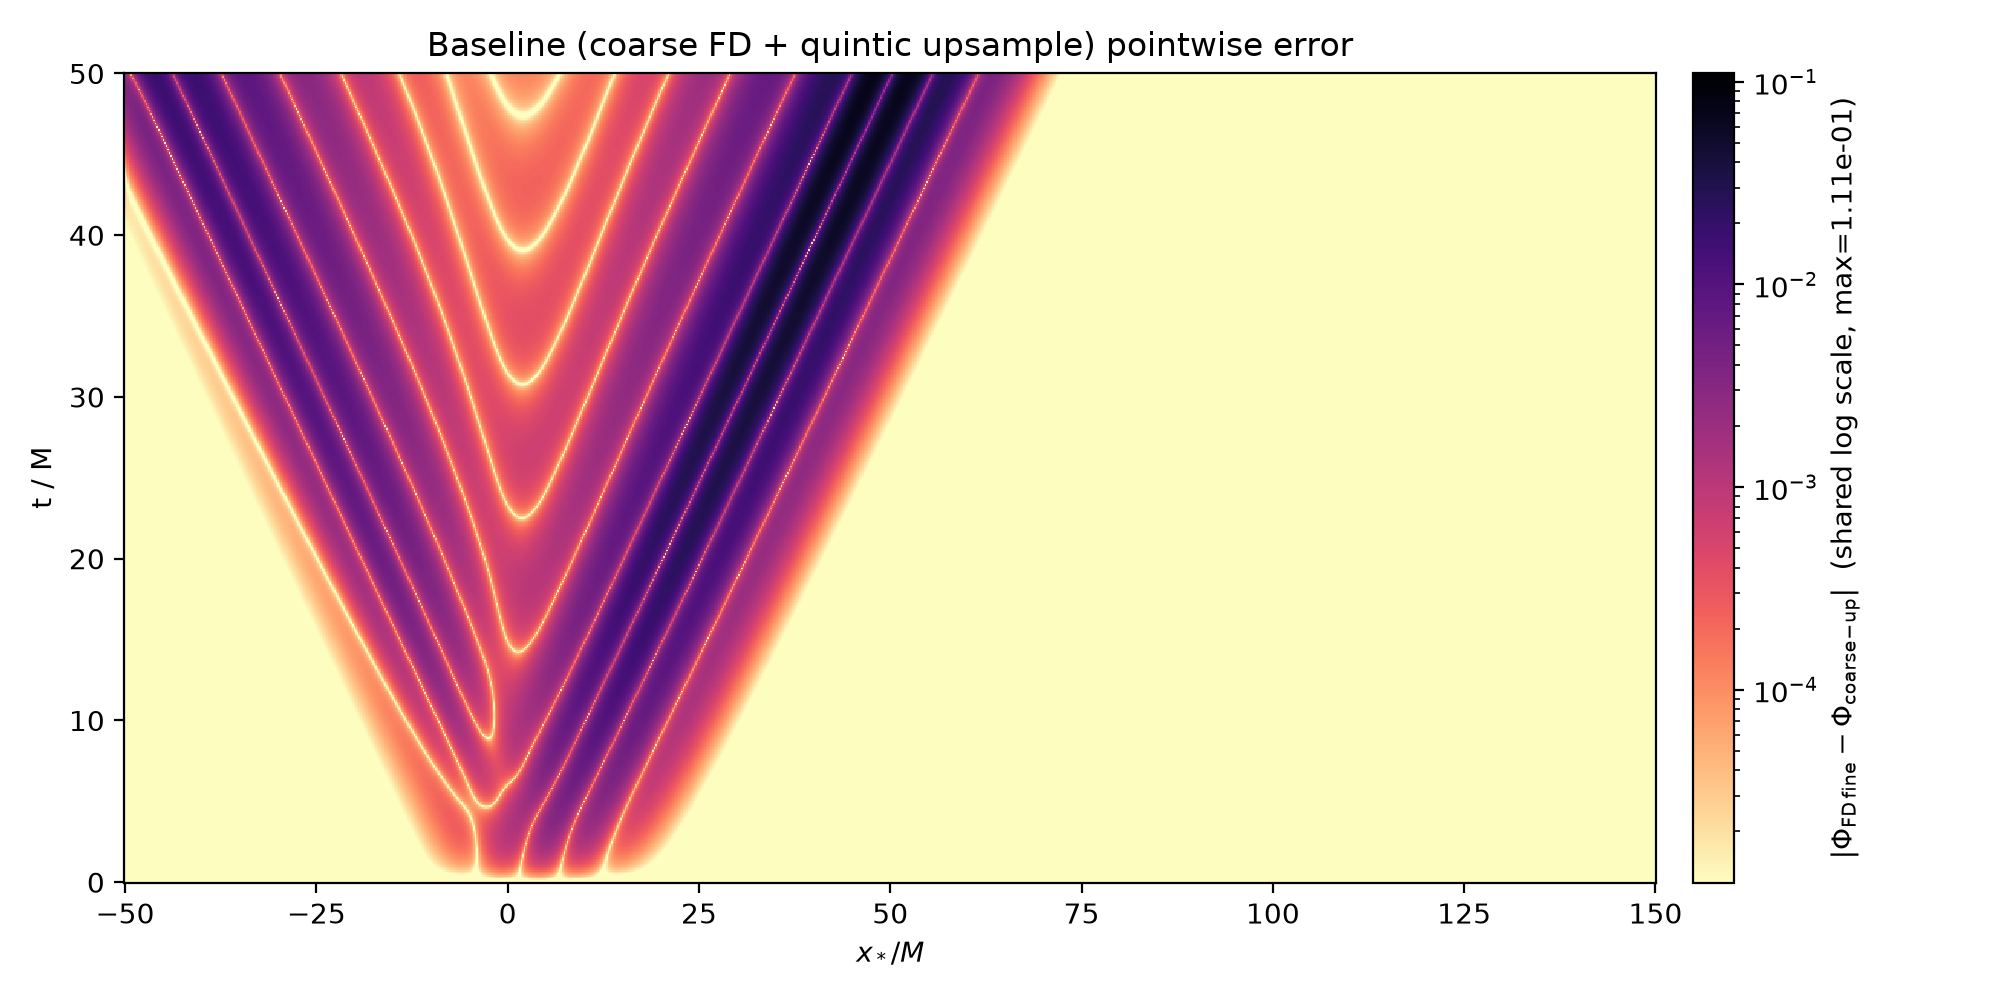
\includegraphics[width=0.92\textwidth]{../outputs/hybrid/fno_sw_gate_s1em3/figs/hybrid_pointwise_error_baseline.png}
\caption{Coarse-up baseline pointwise error on the canonical
BH, plotted on the same shared colour scale as
Fig.~\ref{fig:hyb-heatmap}. The second-order dispersion
signature of the under-resolved $k = 4$ coarse prior plus
quintic upsampling is visible as narrow characteristics tracing
the outgoing-wave caustics; compare the hybrid map of
Fig.~\ref{fig:hyb-heatmap} on the same scale.}
\label{fig:hyb-heatmap-base}
\end{figure}

\paragraph{The gradient gate.} The gate of
Eq.~\eqref{eq:hyb-gate} rests on the hypothesis that the
coarse-prior error is large exactly where the prior gradient
is large; the per-cell scatter on the canonical BH confirms
this with a log--log Pearson correlation of $r = 0.917$, and a
decile stratification shows the hybrid's gain following the
gate --- a factor $14.1$ error reduction in the top gradient
decile, declining monotonically to unity below the median
(Appendix~\ref{app:supp-gate}). The gate scale $s = 10^{-3}$
is derived from the prior gradient distribution alone and sits
within $2\%$ of the field-RMSD optimum
(App.~\ref{app:gate-scale}). The gate also protects the
regions the prior already resolves: over the $60.5\%$ of the
domain with prior error below $10^{-5}$, spurious network
output is held at the $10^{-6}$ level, so the global-field
gain does not pollute the QNM-bearing late-time tail.

\paragraph{Population field accuracy.} Averaged over the 100-BH
in-distribution test set, the gridwise field MSE is
$9.38\times 10^{-7}$ for the hybrid and $7.76\times 10^{-5}$
for the coarse-up baseline, a factor-of-$82$ reduction
($0.648\%$ vs $6.11\%$ relative $L^{2}$) --- consistent across
the whole training distribution rather than an artefact of the
canonical draw.

\begin{figure}[!htbp]
\centering
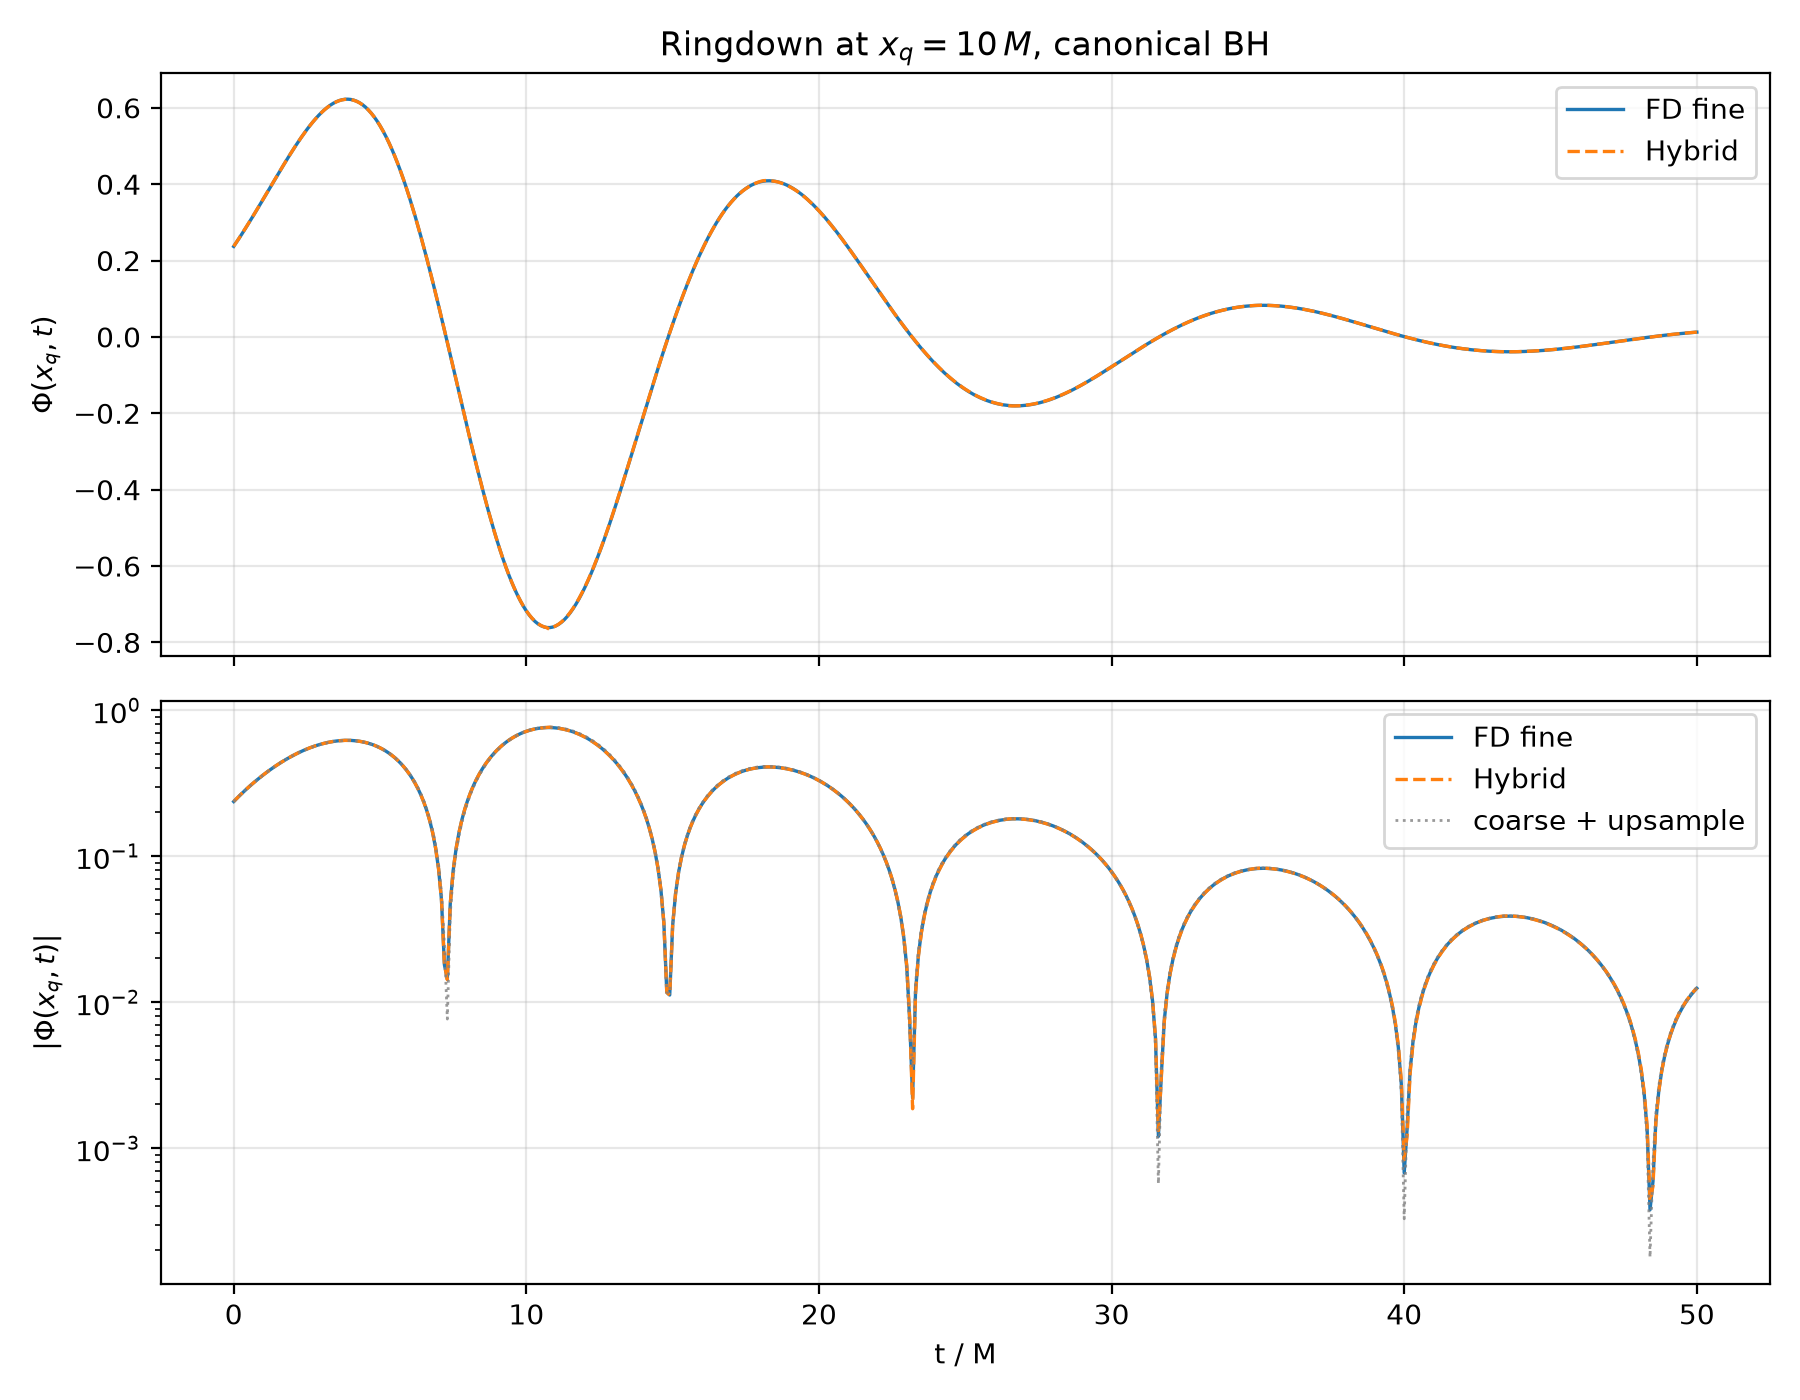
\includegraphics[width=0.80\textwidth]{../outputs/hybrid/fno_sw_gate_s1em3/figs/hybrid_ringdown_xq10.png}
\caption{Observer-slice waveform $\Phi(\xq{=}10, t)$ on the
canonical BH. Top: linear scale. Bottom: $\log_{10}|\Phi|$
scale with the fine FD reference (blue), the hybrid prediction
(orange dashed) and the coarse-up baseline (grey dotted)
overlaid. The canonical plateau extractions of
Figs.~\ref{fig:hyb-plateau-m4} and~\ref{fig:hyb-plateau-m5}
are read from these time series, and
Table~\ref{tab:hyb-canonical} reports the population medians
of the same three-way comparison.}
\label{fig:hyb-ringdown-xq2}
\end{figure}

\paragraph{QNM extraction.} The relevant test for a surrogate is
whether it reproduces the spectroscopy of the fine reference it
approximates. Table~\ref{tab:hyb-canonical} reports the
population-median extraction against that reference at the
common observer over the model's full $[10,100]\,M$ evolution;
the ringdown overlay is Fig.~\ref{fig:hyb-ringdown-xq2} and the
M4/M5 plateau construction is illustrated in
Figs.~\ref{fig:hyb-plateau-m4} and~\ref{fig:hyb-plateau-m5}. On
the primary M4 plateau the hybrid recovers $\omega$ to $0.152\%$
and $\tau$ to $0.528\%$, against the reference's own $0.064\%$
and $0.092\%$ --- the \emph{extractor floor}, the accuracy the
extraction method reaches on the exact field. The hybrid tracks
the reference in frequency to within a tenth of a percentage
point; its damping-time error, however, sits above that floor,
because the network's residual leaves a small incoherent
component in the late ring that the plateau fit cannot average
out. The single canonical draw forms no stable M4 plateau
across the full window, so the QNM is reported on the $100$-BH
population; the coarse prior is the surrogate's field input
(Sec.~\ref{sec:res-hyb}), not a spectroscopic benchmark.

\begin{table}[!htbp]
\centering
\caption{QNM extraction at the common observer $\xq = 10\,M$,
window $t \in [10, 100]\,M$, reported as the
\emph{median} percentage error over the 100-BH in-distribution
test set: hybrid prediction against the fine FD reference it
approximates. Five extraction methods of Sec.~\ref{sec:qnm-methods},
with the plateau scans of
Sec.~\ref{sec:plateau} for M4 and M5. Entries are median
percentage errors of $\omega$ and $\tau$ against the Leaver
reference $(\omega_{0} M, \tau_{0}/M) = (0.3737, 11.241)$. The
hybrid tracks the reference in frequency; its damping-time
error sits above the reference floor, limited by the residual
in the late ring, not by the plateau estimator. Bold entries are
the primary values under the reporting convention of
Sec.~\ref{sec:reporting}.}
\label{tab:hyb-canonical}
\small
\setlength{\tabcolsep}{4pt}
\begin{tabular}{@{}lcccc@{}}
\toprule
 & \multicolumn{2}{c}{Hybrid}
 & \multicolumn{2}{c}{Fine FD reference} \\
\cmidrule(lr){2-3}\cmidrule(lr){4-5}
Method & $|\Delta\omega|\%$ & $|\Delta\tau|\%$
       & $|\Delta\omega|\%$ & $|\Delta\tau|\%$ \\
\midrule
M1 (FFT $+$ log-line)        & $0.423$ & $1.42$ & $0.421$ & $1.16$ \\
M2 (1-mode NLS)              & $2.191$ & $10.3$ & $2.153$ & $10.3$ \\
M3 (ESPRIT $K{=}4$)          & $1.468$ & $7.98$ & $1.444$ & $7.93$ \\
M4 (1-D plateau)             & $\mathbf{0.152}$ & $\mathbf{0.528}$ & $0.064$ & $0.092$ \\
M5 (2-D plateau)             & $0.250$ & $1.37$ & $0.138$ & $1.09$ \\
\bottomrule
\end{tabular}
\end{table}

\begin{figure}[!htbp]
\centering
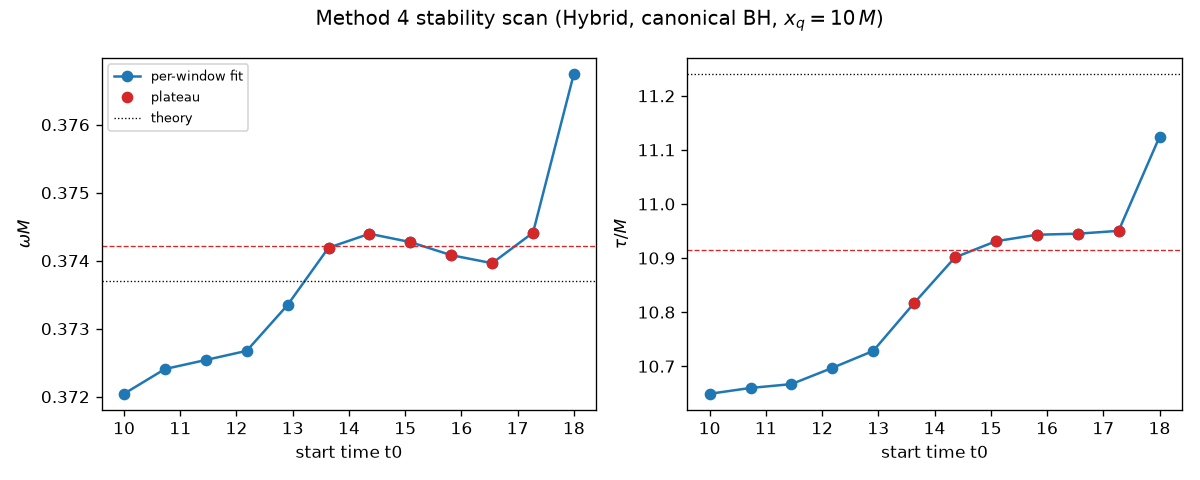
\includegraphics[width=0.80\textwidth]{../outputs/hybrid/fno_sw_gate_s1em3/figs/hybrid_plateau_m4_xq10.png}
\caption{M4 1-D plateau scan on the hybrid prediction at the
canonical BH and $\xq = 10\,M$. Per-window two-mode NLS fits
(blue circles) on $t_{0} \in [10, 18]\,M$ at fixed
$\tend = 50\,M$; the red circles mark the contiguous plateau
block of $6$ start times on $t_{0} \in [13.6, 17.3]\,M$ used to
form the canonical M4 estimate. Black
dotted lines mark the Leaver reference values $\omega = 0.3737$
and $\tau = 11.241\,M$.}
\label{fig:hyb-plateau-m4}
\end{figure}

\paragraph{Training history.} A single Adam phase reduces the
validation MSE on the gated Richardson residual from
$3.6\times 10^{-4}$ to $1.8\times 10^{-6}$ over $100$ epochs,
with train and validation tracking together
(Fig.~\ref{fig:hyb-loss}).

\begin{figure}[!htbp]
\centering
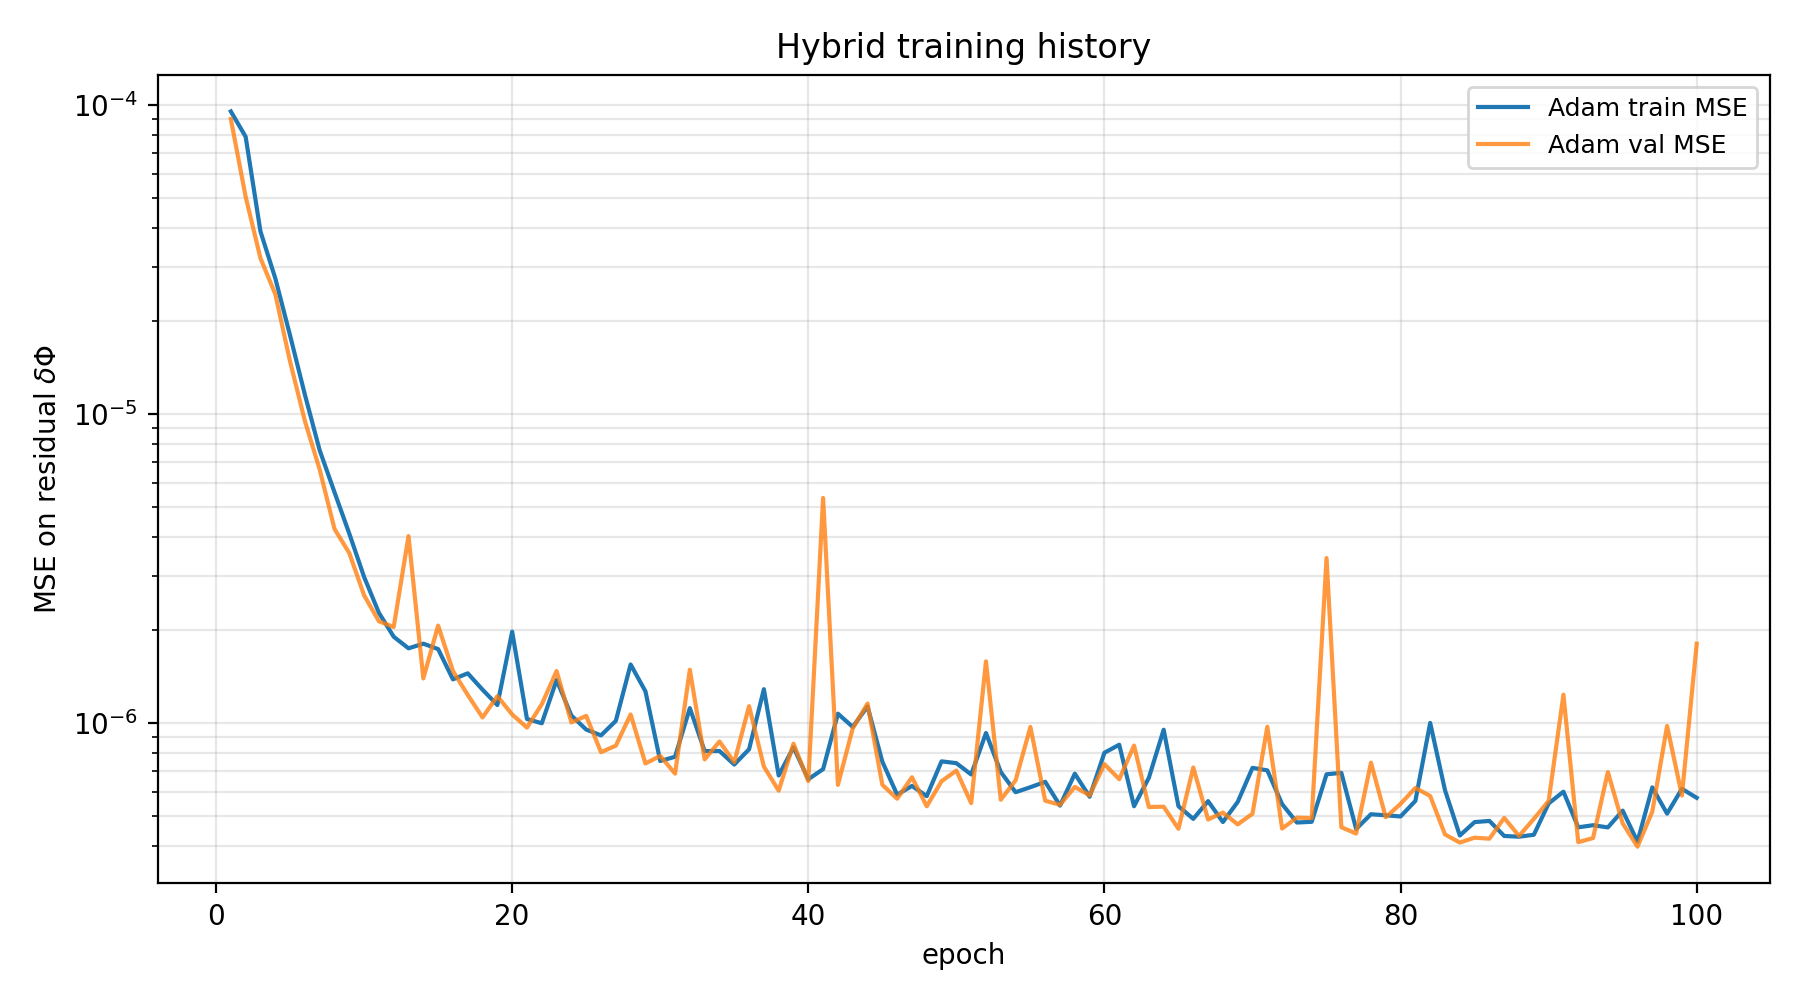
\includegraphics[width=0.85\textwidth]{../outputs/hybrid/fno_sw_gate_s1em3/figs/hybrid_loss.png}
\caption{Hybrid surrogate training history: per-epoch train and
validation MSE on the gated Richardson residual over $100$ Adam
epochs.}
\label{fig:hyb-loss}
\end{figure}

\FloatBarrier

% ==============================================================
\subsection{Generalisation to Kerr}
\label{sec:res-kerr}

The final experiment asks whether the hybrid construction is
tied to the Schwarzschild geometry. We retrain the surrogate on
a $128$-black-hole test set drawn from a Sobol sequence in
dimensionless spin $a/M \in [0, 0.95]$, evolving the
hyperboloidal Teukolsky field of Sec.~\ref{sec:teukolsky-problem} and
targeting the fundamental $(\ell, m, n) = (4, 2, 0)$ mode.
Table~\ref{tab:kerr-summary} collects the field and frequency
accuracy by spin bin.

\paragraph{Field.} Across the test set the coarse prior carries
a median relative $L^{2}$ field error of $59.5\%$: at low
resolution the hyperboloidal wavefront is badly
under-resolved. The hybrid reduces this to $0.78\%$, a factor
of $77$, and the error stays nearly flat across spin --- from
$0.70\%$ at low spin to $1.08\%$ near extremality
(Table~\ref{tab:kerr-summary}) --- so a single amortised
operator absorbs almost the entire spin dependence of the
field. The label-free Richardson target itself sits at
$0.008\%$, confirming that the FNO, not the reference, sets the
floor. Figure~\ref{fig:kerr-ringdown} overlays the
reconstructed ringdown at $\scri$ against the fine reference
for a representative $a/M = 0.7$ black hole, and
Fig.~\ref{fig:kerr-pointwise} shows the coarse solve's error
concentrated in the high-amplitude burst, which the residual
correction removes.

\paragraph{Frequency.} The amortisation is clearest at high
spin, where the coarse prior degrades fastest. For
$a/M \ge 0.8$ ($20$ black holes) the best-of-suite prior
frequency error is $4.71\%$, which the hybrid cuts to $0.38\%$
--- a $12\times$ improvement --- approaching the fine-solve
floor of $0.02\%$ (Table~\ref{tab:kerr-summary},
Fig.~\ref{fig:kerr-vs-spin}). Pooled over all spins the median
frequency error falls from $0.59\%$ to $0.33\%$, with the fine
solve at $0.05\%$. The correction is largest exactly where it
is needed: at moderate spin the prior is already sub-percent
and the hybrid tracks it, whereas near extremality --- where
the near-horizon oscillation of Eq.~\eqref{eq:kerr-rescale} is
strongest and the coarse grid fails --- the hybrid recovers
more than an order of magnitude.

\paragraph{Damping time.} The damping time is the harder
channel (Fig.~\ref{fig:kerr-vs-spin}c), exactly as for the
Zerilli surrogate (Sec.~\ref{sec:res-hyb}). Pooled over spin the
hybrid $\tau$
error ($1.52\%$) exceeds that of the coarse prior ($0.52\%$),
while the fine solve ($0.27\%$) shows that the residual
correction --- tuned to the field and its leading oscillation
--- does not consistently sharpen the exponential envelope.
This is the same trade-off seen for Schwarzschild: the operator
restores the phase and amplitude of the field far better than
its slowly varying decay rate, so $\tau$ remains a fine-solve
quantity and the surrogate is a frequency-and-field
accelerator rather than a damping-time estimator.

\paragraph{Verdict.} Taken together, the Kerr experiment shows
that the hybrid concept is geometry-agnostic. The same
coarse-plus-residual construction, retrained without a single
fine-grid field in its loss, transfers from a static
Schwarzschild wave equation to a rotating, complex,
hyperboloidal Teukolsky field and still delivers an
order-of-magnitude field improvement and sub-percent
frequencies across the astrophysical spin range --- a
generalisation that a per-black-hole PINN, retrained from
scratch for every spin, does not provide.

\begin{table}[!htbp]
\centering
\caption{Kerr hybrid surrogate accuracy by spin bin over the
$128$-black-hole test set: bin medians, with the final row the
population median. Field errors are relative $L^{2}$ against the
fine solve, for the coarse prior, the hybrid, and the label-free
Richardson target. Frequency ($|\delta\omega|/\omega$) and
damping-time ($|\delta\tau|/\tau$) errors are the best-of-suite
values for the $(4,2,0)$ mode, with the fine-solve error shown
for reference. The estimator winning most often for the hybrid
is noted below the table
(M3 $=$ selective ESPRIT, cES $=$ complex ESPRIT,
c$\Phi$ $=$ complex-phase fit; Sec.~\ref{sec:teukolsky-problem}).}
\label{tab:kerr-summary}
\footnotesize
\setlength{\tabcolsep}{4pt}
\begin{tabular}{lr rrr rrr rrr}
\toprule
 & & \multicolumn{3}{c}{Field rel-$L^{2}$ (\%)}
   & \multicolumn{3}{c}{$M\omega$ err.\ (\%)}
   & \multicolumn{3}{c}{$\tau/M$ err.\ (\%)} \\
\cmidrule(lr){3-5}\cmidrule(lr){6-8}\cmidrule(lr){9-11}
$a/M$ & $n$ & prior & hybrid & Rich.
      & prior & hybrid & fine
      & prior & hybrid & fine \\
\midrule
$[0.0,0.3]$  & $41$ & $51.2$ & $0.70$ & $0.004$ & $0.63$ & $0.53$ & $0.06$ & $0.56$ & $1.79$ & $0.46$ \\
$[0.3,0.6]$  & $40$ & $59.1$ & $0.70$ & $0.006$ & $0.44$ & $0.27$ & $0.08$ & $0.29$ & $1.67$ & $0.42$ \\
$[0.6,0.8]$  & $27$ & $65.7$ & $0.86$ & $0.013$ & $0.39$ & $0.23$ & $0.04$ & $0.32$ & $1.22$ & $0.16$ \\
$[0.8,0.95]$ & $20$ & $73.6$ & $1.08$ & $0.063$ & $4.71$ & $0.38$ & $0.02$ & $1.43$ & $2.19$ & $0.02$ \\
\midrule
All (median) & $128$ & $59.5$ & $0.78$ & $0.008$ & $0.59$ & $0.33$ & $0.05$ & $0.52$ & $1.52$ & $0.27$ \\
\bottomrule
\end{tabular}

\smallskip
{\footnotesize\raggedright Dominant hybrid estimator by
ascending spin bin --- $M\omega$: cES, M3, M3, M3 (M3 overall);
$\tau/M$: cES, cES, M3, c$\Phi$ (cES overall).\par}
\end{table}

\begin{figure}[!htbp]
\centering
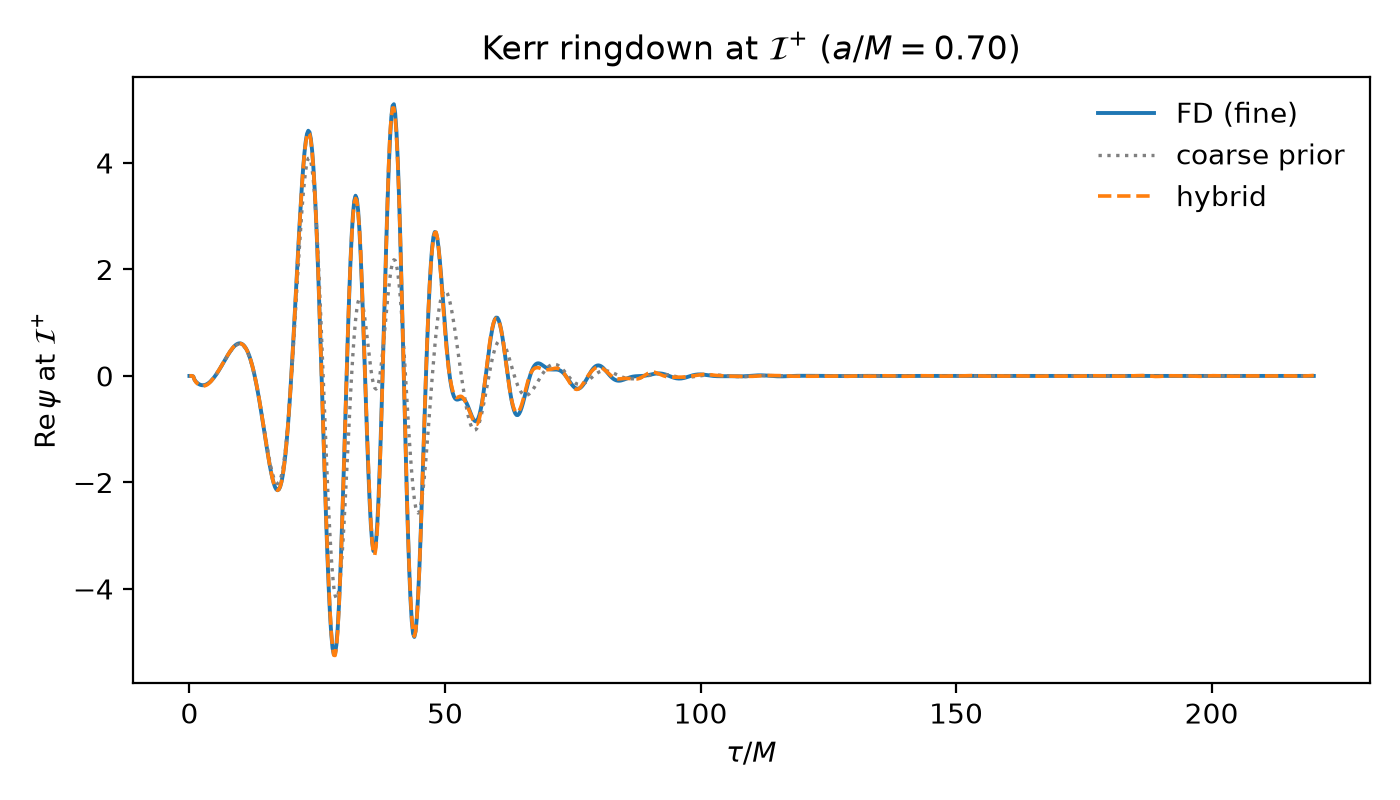
\includegraphics[width=0.82\textwidth]{../outputs/kerr/figs/hybrid_ringdown_scri.png}
\caption{Kerr ringdown at null infinity $\scri$ for a
representative $a/M = 0.7$ black hole. The hybrid (orange,
dashed) overlays the fine reference (blue, solid), whereas the
coarse prior (grey, dotted) departs from it in amplitude and
phase through the peak of the burst.}
\label{fig:kerr-ringdown}
\end{figure}

\begin{figure}[!htbp]
\centering
\begin{subfigure}[t]{0.49\textwidth}
\centering
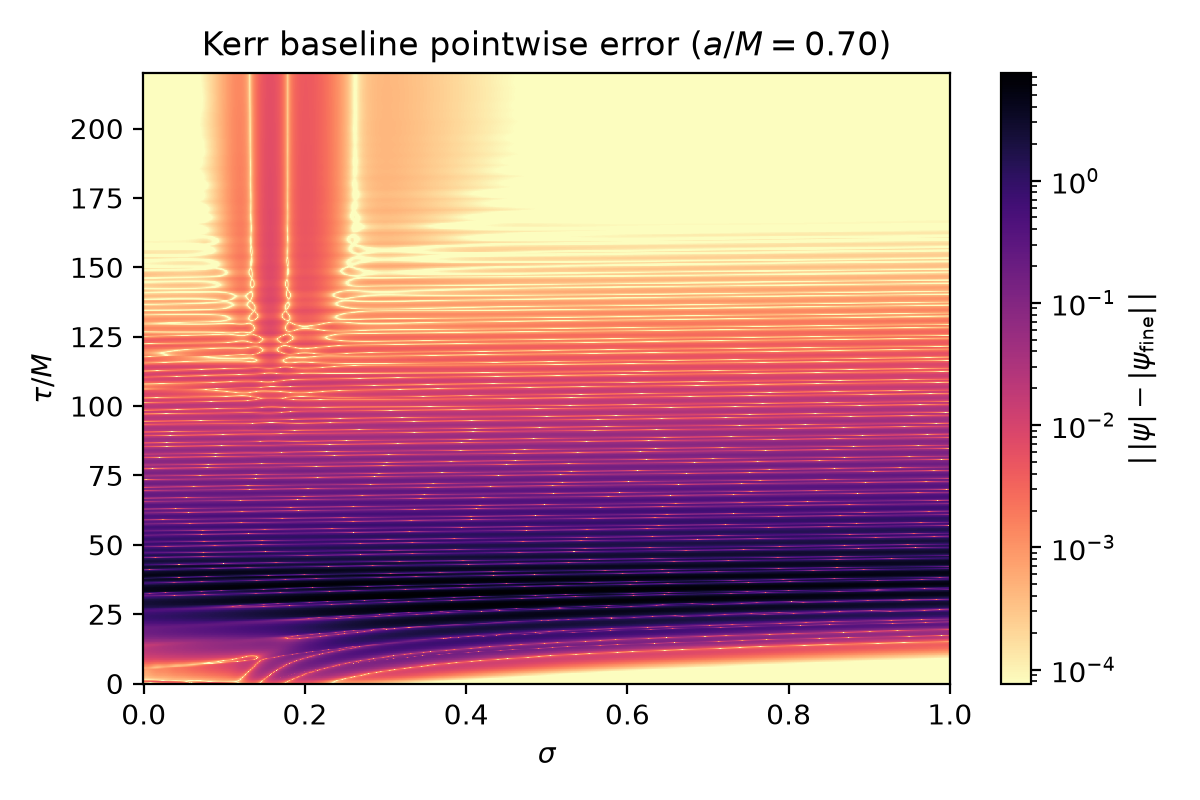
\includegraphics[width=\textwidth]{../outputs/kerr/figs/hybrid_pointwise_error_baseline.png}
\subcaption{Coarse prior.}
\end{subfigure}
\hfill
\begin{subfigure}[t]{0.49\textwidth}
\centering
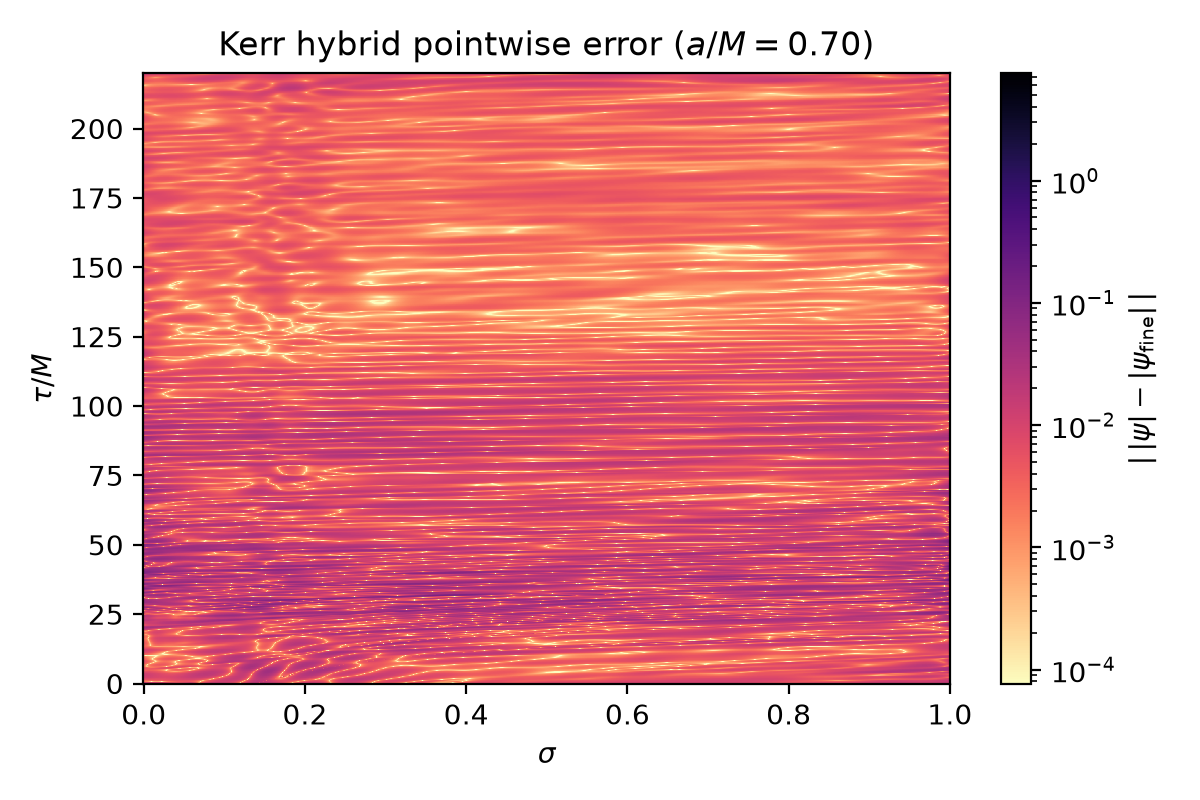
\includegraphics[width=\textwidth]{../outputs/kerr/figs/hybrid_pointwise_error_hybrid.png}
\subcaption{Hybrid.}
\end{subfigure}
\caption{Pointwise field error over the compactified domain
$(\sigma, \tau)$, both panels on the same logarithmic colour
scale. The coarse prior (a) concentrates its error in the
high-amplitude burst phase (early $\tau$); the residual FNO (b)
removes that burst-phase structure, leaving a much lower
residual across the domain.}
\label{fig:kerr-pointwise}
\end{figure}

\begin{figure}[!htbp]
\centering
\begin{subfigure}[t]{0.49\textwidth}
\centering
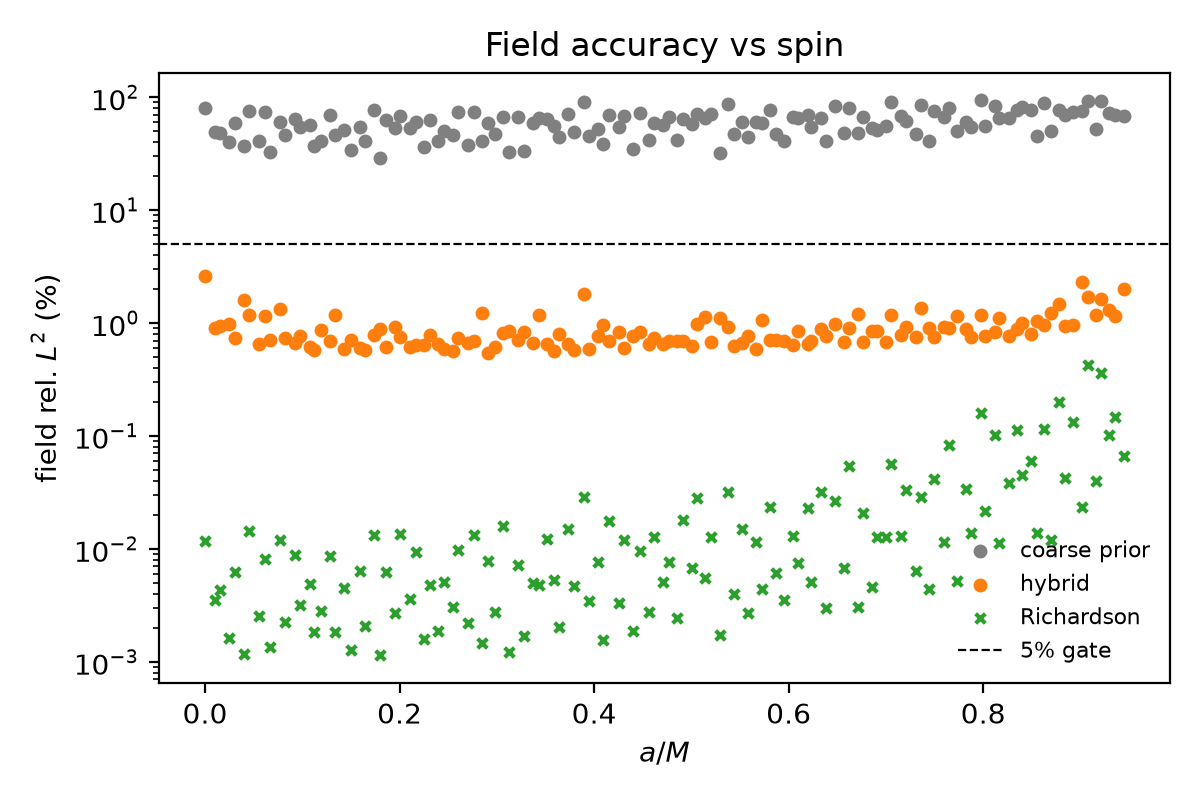
\includegraphics[width=\textwidth]{../outputs/kerr/figs/hybrid_field_vs_spin.png}
\subcaption{Field error.}
\end{subfigure}
\hfill
\begin{subfigure}[t]{0.49\textwidth}
\centering
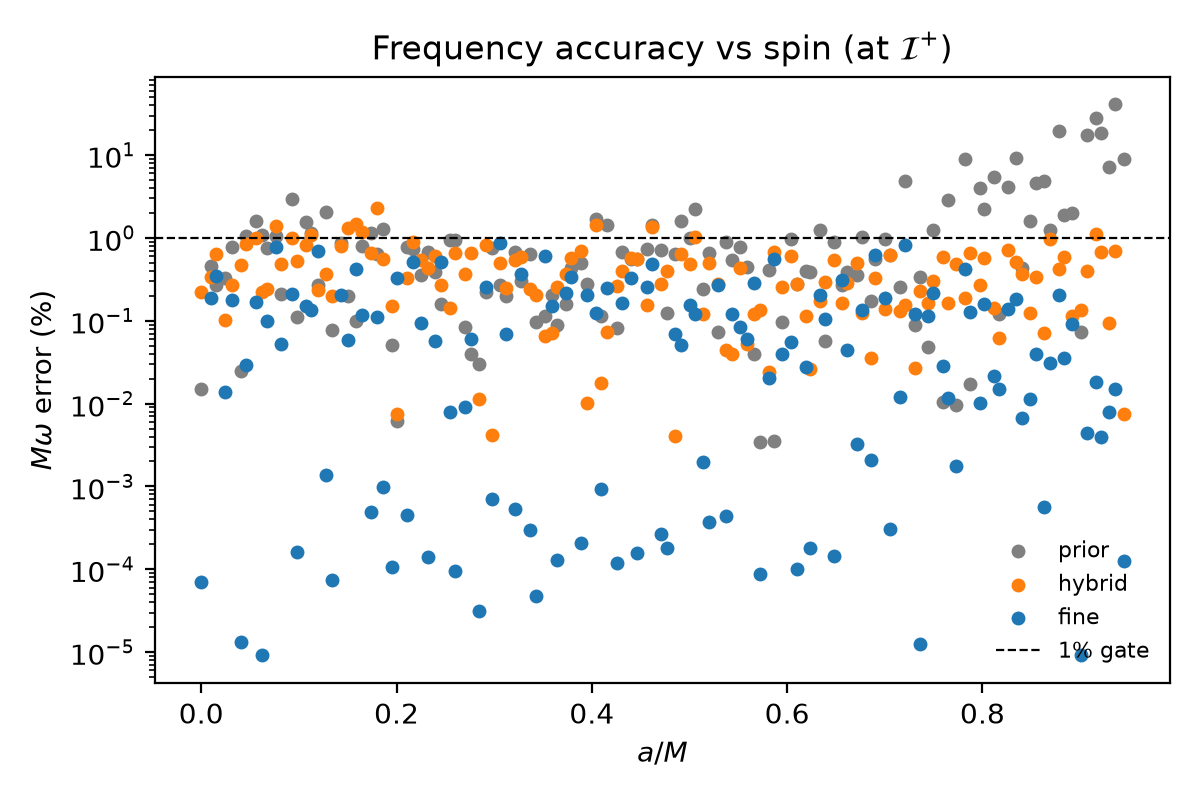
\includegraphics[width=\textwidth]{../outputs/kerr/figs/hybrid_qnm_vs_spin.png}
\subcaption{Frequency error.}
\end{subfigure}

\vspace{0.6em}
\begin{subfigure}[t]{0.49\textwidth}
\centering
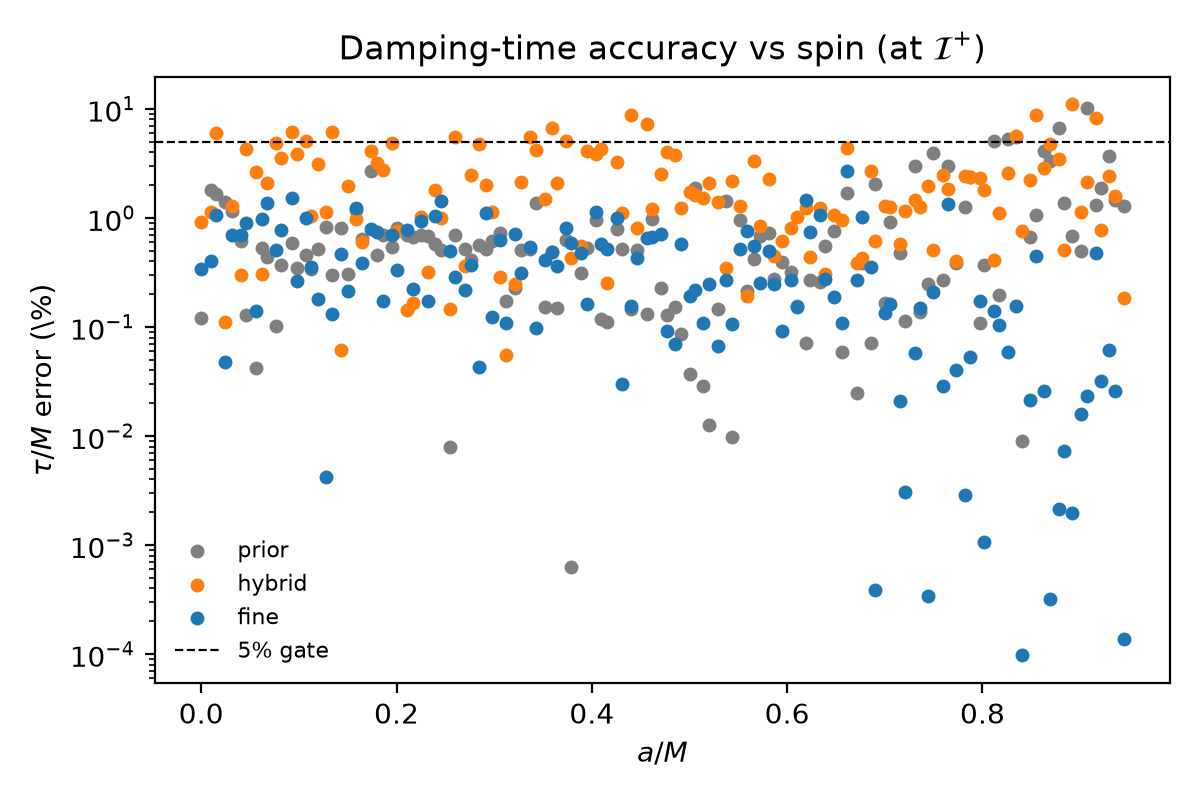
\includegraphics[width=\textwidth]{../outputs/kerr/figs/hybrid_tau_vs_spin.png}
\subcaption{Damping-time error.}
\end{subfigure}
\caption{Best-of-suite accuracy versus spin (coarse prior grey,
hybrid orange; fine reference blue in (b) and (c), label-free
Richardson target green in (a)). (a)~The hybrid field error is
flat across $a/M$ while the coarse prior grows towards
extremality. (b)~The prior frequency error spikes for
$a/M \gtrsim 0.8$, where the hybrid recovers more than an order
of magnitude and approaches the fine-solve floor. (c)~The
damping time is the exception: the hybrid does not improve on
the prior and stays well above the fine floor, as discussed in
the text.}
\label{fig:kerr-vs-spin}
\end{figure}

\FloatBarrier
